\chapter{Manifolds in $\R^n$}

\section{k-dimensional Parallelopiped in $\R^n$}

\begin{lemma}
    Let $W$ be a linear subspace of $\R^n$ of dimension $k$. Then there is an orthonormal basis for $\R^n$ whose first $k$ elements form a basis for $W$.
\end{lemma}

\begin{theorem}
    Let $W$ be a k-dimensional linear subspace of $\R^n$. There is an orthogonal transformation $h:\R^n\longrightarrow\R^n$ that carries $W$ onto the subspace $\R^k\times0$ of $\R^n$.
\end{theorem}

\begin{definition}
    Given vectors $\vec{x_1},\cdots,\vec{x_k}$ is $\R^n$. 
    Define the n by k matrix $$X=\begin{bmatrix}
        \vec{x_1} & \cdots & \vec{x_k}
    \end{bmatrix}$$
    we define the \underline{k-dimensional volume} of the parallelopiped $\mathcal{P}(\vec{x_1},\cdots,\vec{x_k})$ to be 
    $$V(\vec{x_1},\cdots,\vec{x_k})=\sqrt{\det(X^T\cdot X)}$$
\end{definition}
\noindent\textbf{Example}:
\begin{itemize}
    \item Consider two independent vectors $\vec{a},\vec{b}$ in $\R^3$. Define the 3 by 2 matrix $$X=\begin{bmatrix}
        \vec{a} & \vec{b}
    \end{bmatrix}$$
    Let $\theta$ denote the angle between $\vec{a},\vec{b}$, then 
    \begin{equation*}
        \begin{split}
            V^2(\vec{a},\vec{b}) &= V^2(X)\\
            &= \det(\begin{bmatrix}
                \norm{\vec{a}}^2 & \innerp{\vec{a}}{\vec{b}}\\
                \innerp{\vec{b}}{\vec{a}} & \norm{\vec{b}}^2
            \end{bmatrix})\\
            &= \norm{\vec{a}}^2 \norm{\vec{b}}^2(1-\cos^2\theta)\\
            &= \norm{\vec{a}}^2 \norm{\vec{b}}^2\sin^2\theta
        \end{split}
    \end{equation*}
    \begin{figure}[H]
        \centering
        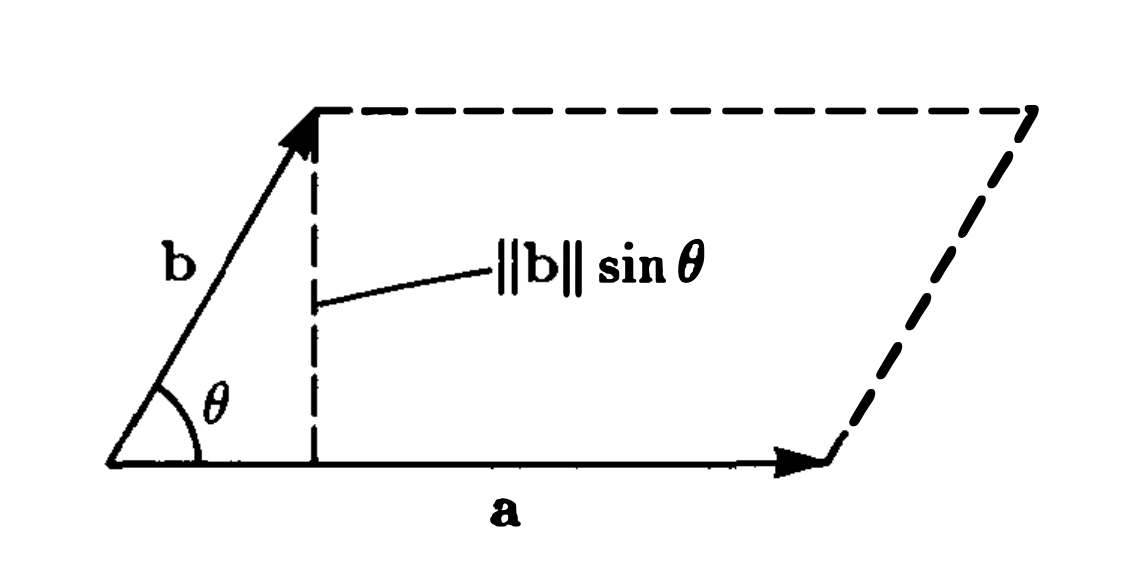
\includegraphics[scale=0.3]{images/Screenshot 2023-01-16 at 02.13.22.png}
        \caption{picture of 2-dimensional volume in $\R^3$}
    \end{figure}
\end{itemize}

\begin{theorem}[Properties of k-dim volume in $\R^n$]\
    \begin{enumerate}
        \item If $h:\R^n\longrightarrow\R^n$ is an orthogonal transformation, then $$V(h(\vec{x_1}),\cdots,h(\vec{x_k}))=V(\vec{x_1},\cdots,\vec{x_k})$$
        \item If $\vec{y_1},\cdots,\vec{y_k}$ belong to the subspace $\R^k\times 0$ of $\R^n$, such that $$\vec{y_i}=\begin{bmatrix}
            \vec{z_i}\\
            \vec{0}
        \end{bmatrix}$$
        where $\vec{z_i}\in\R^k$, $\vec{0}\in\R^{n-k}$, then 
        $$V(\vec{y_1},\cdots,\vec{y_k})=|\det(\begin{bmatrix}
            \vec{z_1} & \cdots & \vec{z_k}
        \end{bmatrix})|$$
        \item $\vec{x_1},\cdots,\vec{x_k}$ are linear dependent if and only if $V(\vec{x_1},\cdots,\vec{x_k})\neq0$
    \end{enumerate}
\end{theorem}

\begin{definition}
    Let $\vec{x_1},\cdots,\vec{x_k}$ be vectors in $\R^n$ with $k\leq n$. Define the n by k matrix $$X=\begin{bmatrix}
        \vec{x_1} & \cdots \vec{x_k}
    \end{bmatrix}$$
    Define an ascending k-tuple from $\{1,\cdots,n\}$ $$I=(i_1,\cdots,i_k)$$
    where $1\leq i_1\leq i_2\leq \cdots \leq i_k\leq n$
    Finally, we define the k by k matrix $X_I$ or $X(i_1,\cdots,i_k)$ to be the submatrix of $X$ consisting of rows $i_1,\cdots,i_k$.
\end{definition}

\begin{theorem*}
    Let $X$ be an n by k matrix with $k\leq n$. Then
    $$V^2(X)=\sum_{[I]}[\det(X_I)]^2$$
    where the symble $[I]$ indicates that the summaton extends over all ascending k-tupes from $\{1,\cdots,n\}$.
\end{theorem*}
\noindent\textbf{Remark}:
\begin{itemize}
    \item This theorem may be thought of as a Pythagorean theorem for k-volume. It states that the square of the volume of a k-parallelopiped $\mathcal{P}$ in $\R^n$ is equal to the sum of the squares of the volumes of the k-parallelopipeds obtained by projecting $\mathcal{P}$ onto the various coordinate k-planes of $\R^n$.
    \item Consider the following picture of a 2-parallelopiped(parallelogram) in $\R^3$.
    \begin{figure}[H]
        \centering
        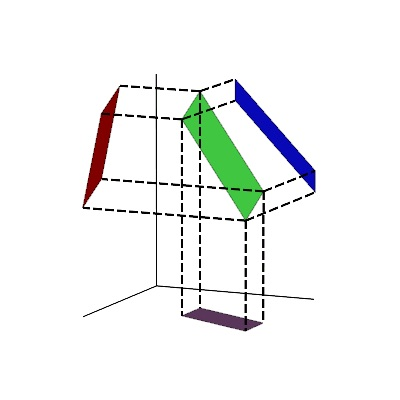
\includegraphics[scale=0.6]{images/vectors_66.jpeg}
        \caption{a 2-parallelopiped(parallelogram) in $\R^3$}
    \end{figure}
    Let $V$ denotes the volume of the 2-parallelopiped, which is the green part. Let $V_r,V_b,V_p$ denotes the volume of the red, blue, purple part respectively.
    This theorem tells us $$V^2=V_r^2+V_b^2+V_p^2$$
\end{itemize}

\section{Parametrized Manifold in $\R^n$}

\begin{definition}
    Let $k\leq n$. Let $A$ be open in $\R^k$, and let $\alpha:A\longrightarrow \R^n$ be a map of class $C^r$.
    The set $Y=\alpha(A)$, together with the map $\alpha$, constitute what is called \underline{parametrized-manifold} of dimension $k$. 
    We denote this parametrized-manifold by $Y_{\alpha}$ and we define the \underline{(k-dimensional) volume} of $Y_{\alpha}$ by the equation
    $$v(Y_{\alpha})=\int_AV(D\alpha)$$
\end{definition}
\noindent\textbf{Remark}:
\begin{itemize}
    \item Consider $A$ is the interior of a closed rectangle $Q$ in $\R^k$. Let $P$ be a partition of the rectangle $Q$.
    Consider one of the very small subrectangles $$R=[a_1,a_1+h_1]\times\cdots\times[a_k,a_k+h_k]$$
    This subtangle is maped to a curved rectangle $\alpha(R)$ in $\R^n$. Since the subrectangle is very very small, and the continuous function $\alpha$ has the locally linearity property, so the curved rectangle $\alpha(R)$ can be considered as a very small parallelopiped.
    \begin{figure}[ht]
        \centering
        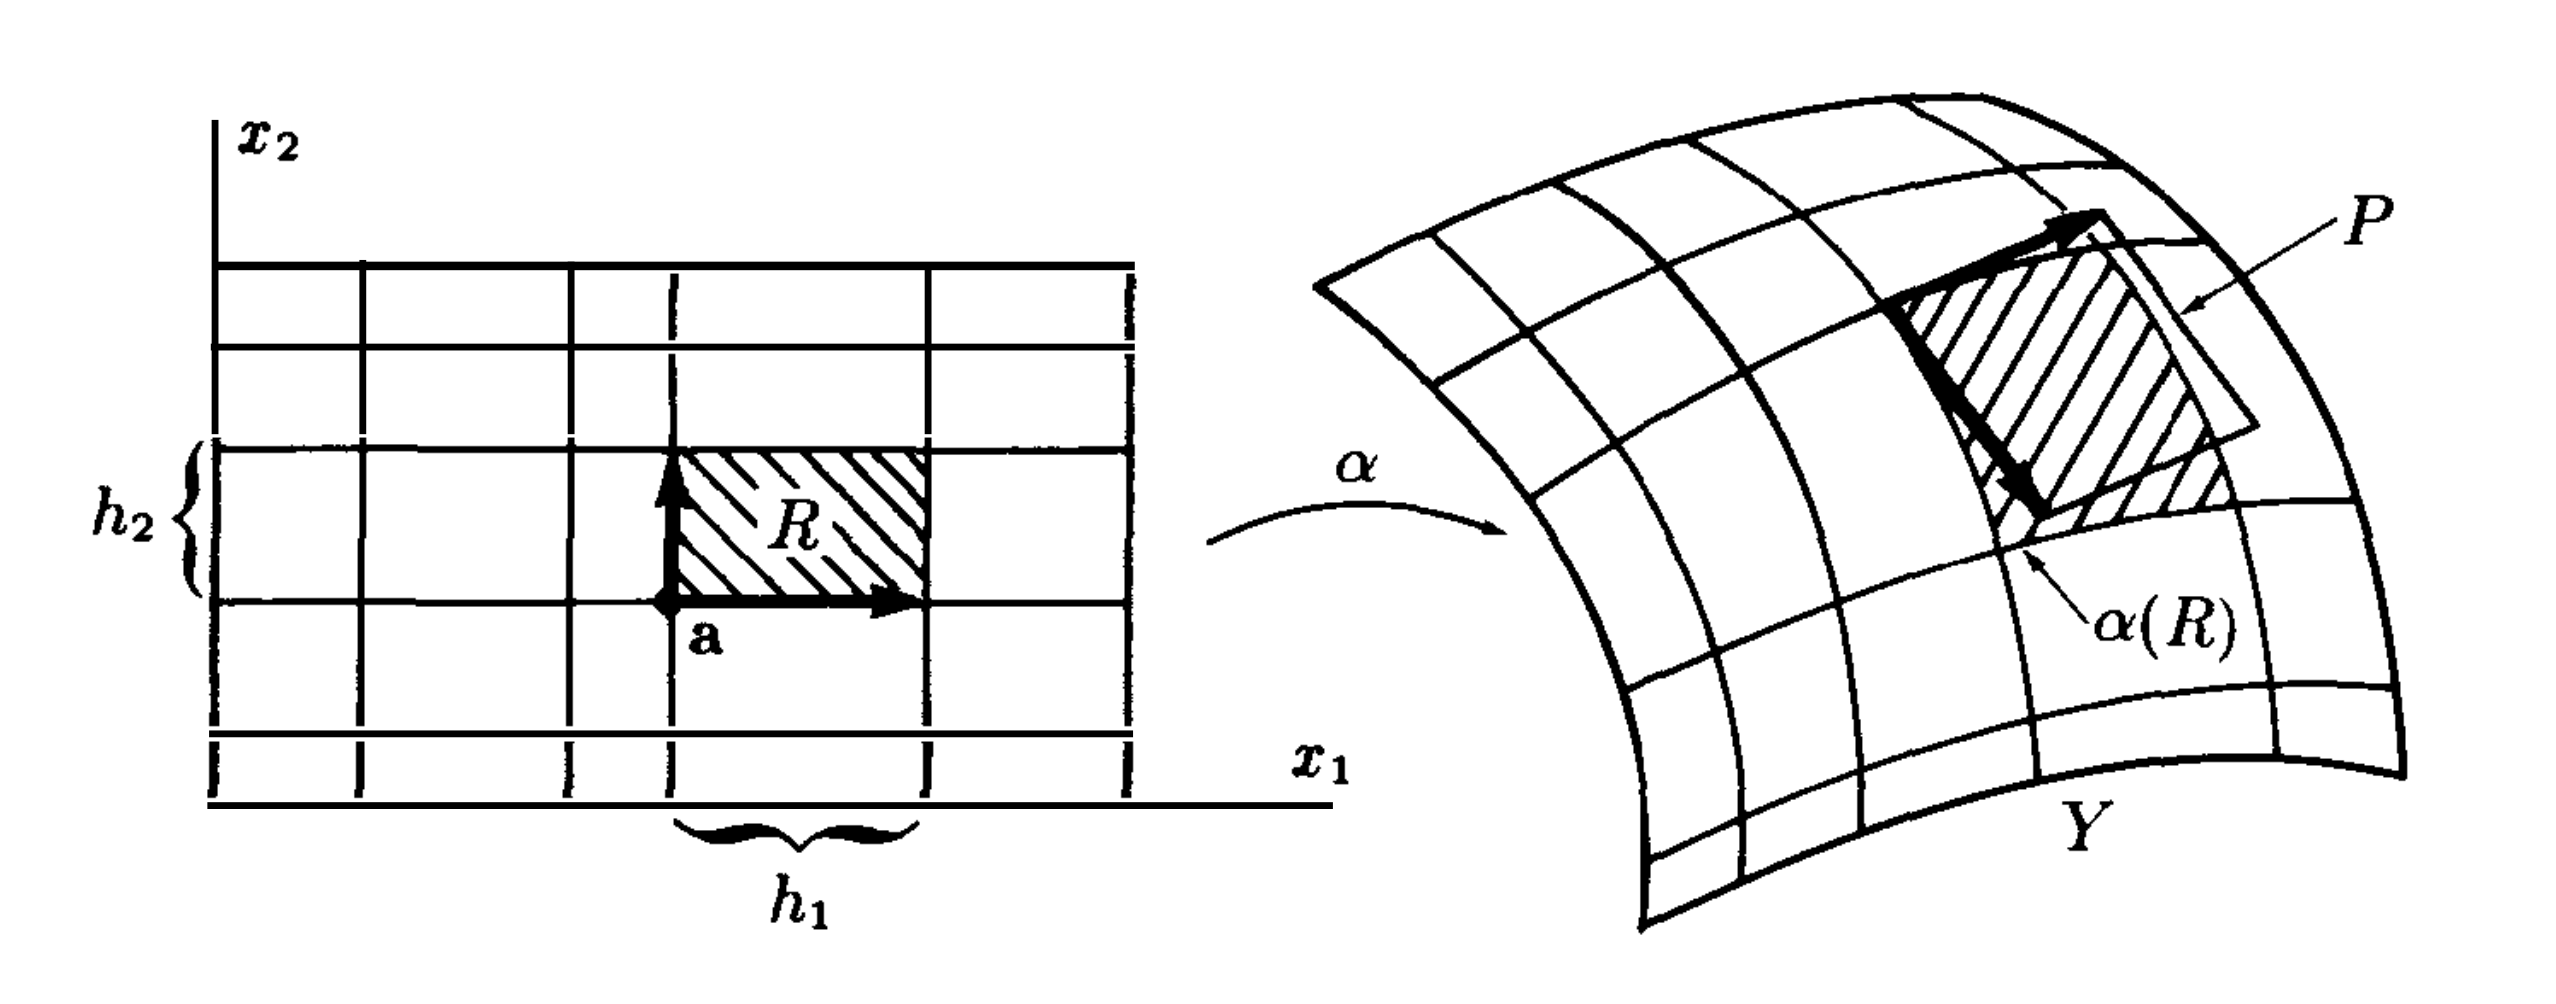
\includegraphics[scale=0.3]{images/Screenshot 2023-01-18 at 13.34.54.png}
        \caption{$\alpha:Int(Q)\subset\R^2\to\R^n$}
    \end{figure}
    \item For the point $\vec{a}=(a_1,\cdots,a_k)$, the jacobian matrix(total derivative) $D\alpha(\vec{a})$ is the linear approximation of the transformation $\alpha$ at the point $\vec{a}$.
    So the volume of the parallelopiped $\alpha(R)$ is $$V(D\alpha(\vec{a})h_1\vec{e_1},\cdots,D\alpha(\vec{a})h_k\vec{e_k})=(h_1\times\cdots\times h_k)V(D\alpha(\vec{a}))=V(D\alpha(\vec{a}))\cdot v(R)$$
    Then we sum over all subrectangles $R$ determined by $P$ to get the approximation of the volume of $Y_{\alpha}(A)$ $$\sum_{R}V(D\alpha)v(R)$$
    \item As the partition gets more and more finer, the summation becomes the integral over $A$, so we get
    $$v(Y_{\alpha})=\int_AV(D\alpha)$$
\end{itemize}

\begin{definition}
    Let $k\leq n$. Let $A$ be open in $\R^k$, and let $\alpha:A\longrightarrow \R^n$ be a map of class $C^r$. Let $Y=\alpha(A)$.
    Let $f:Y\longrightarrow\R$ be a real-valued continuous function. We define the \underline{integral} of $f$ over $Y_{\alpha}$ \underline{with respect to volume}, by the equation
    $$\int_{Y_{\alpha}}f\di V=\int_A(f\circ \alpha)V(D\alpha)$$
\end{definition}
\noindent\textbf{Remark}:
\begin{itemize}
    \item $\di V$ can be considered the unit volume of the parametrized-manifold $Y_{\alpha}(A)$. For example. consider $$\alpha:A\subset \R^2\longrightarrow\R^3$$
    The parametrized-manifold $Y_{\alpha}(A)$ is a surfaces in $\R^3$. $\di V$ can be considered the unit area of $Y_{\alpha}(A)$, which is obtained by streching the unit area of $A$ ($\di x \di y$) by $V(D\alpha)$.
    The function $f:Y(A)\longrightarrow\R$ can be thought of the height, so $f\di V$ is the unit volume. Taking the integral over $Y_{\alpha}(A)$ we get the volume we want. This new notation
     corresponds our intuition.
     \item Consider the one dimensional example. Let $\alpha:A\subset\R\longrightarrow B\subset\R$ be a change of variable. The change of variable theorem tells us
     $$\int_Bf(u)\di u=\int_Af(\alpha(x))\alpha'(x)\di x$$
     Similarly, $\di u$ is the new unit length, which is obtained by streching the unit length of $A$ by $\alpha'$.
\end{itemize}

\begin{theorem}[Invariant under reparametrization]
    Let $g:A\longrightarrow B$ be a diffeomorphism of open sets in $\R^k$. Let $\beta:B\longrightarrow\R^n$ be a map of class $C^r$. Let $Y=\beta(B)$.
    Let $\alpha=\beta\circ g$, then $\alpha:A\longrightarrow\R^n$ and $Y=\alpha(A)$. If $f:Y\longrightarrow\R$ is a continnuous function, then $f$ is integrable over $Y_{\alpha}$ if and only if $f$ is integrable over $Y_{\beta}$.
    In this case $$\int_{Y_{\alpha}}f\di V=\int_{Y_{\beta}}f\di V$$
    \begin{figure}[ht]
        \centering
        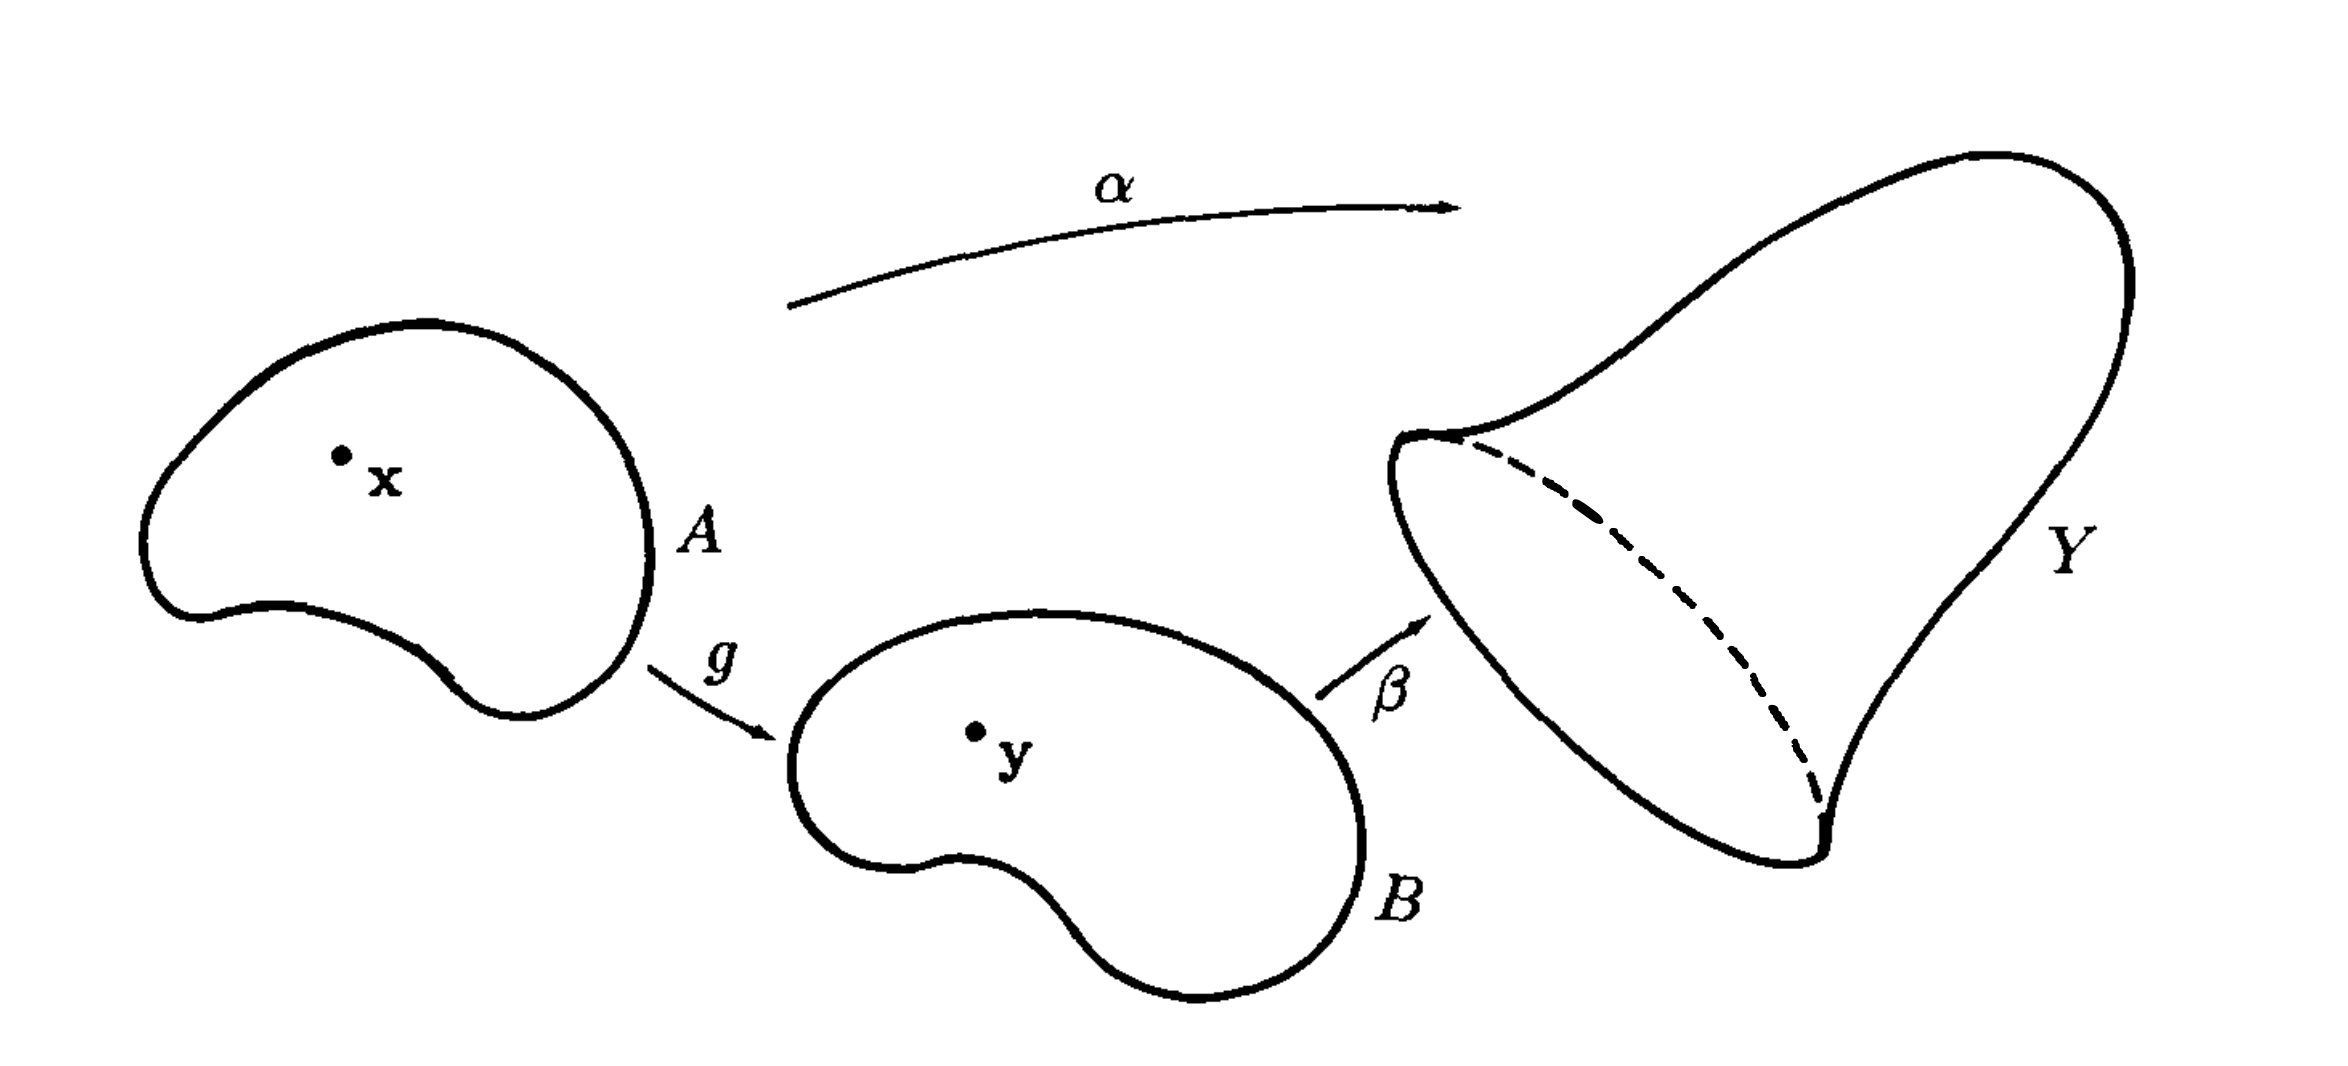
\includegraphics[scale=0.3]{images/Screenshot 2023-01-18 at 14.35.53.png}
        \caption{Invariant under reparametrization}
    \end{figure}
\end{theorem}

\begin{definition}
    Let $A$ be an open set in $\R$. Let $\alpha:A\longrightarrow\R^n$ be a map of class $C^r$. Let $Y=\alpha(A)$. Then $Y_{\alpha}$ is called a \underline{parametrized-curve} in $\R^n$.
    The 1-dimensional volume of $Y_{\alpha}$ is often called its \underline{length}.
\end{definition}

\begin{theorem}
    The length of a parametrized-curve in $\R^n$ is given by the formula
    \begin{equation*}
        v(Y_{\alpha})=\int_AV(D\alpha)=\int_A[(\frac{\di\alpha_1}{\di t})^2+\cdots+(\frac{\di\alpha_n}{\di t})^2]^{\frac{1}{2}}
    \end{equation*}
\end{theorem}
\noindent\textbf{Remark}:
\begin{itemize}
    \item Recall the length of the function $f$ in MAT157 $$l(f)=\int_a^b(1+(f'(t))^2)^{\frac{1}{2}}\di t$$
    In this situation $$\alpha(t)=(t,f(t))$$
    \item Consider a parametrized-curve in $\R^2$ defined by $$\alpha(t)=(a\sin(t),a\cos(t))$$
    Let $A$ be the interval $(0,3\pi)$, can we apply the formula?
    If we apply the formula, then $$\int_{0}^{3\pi}[a^2\sin^2(t)+a^2\cos^2(t)]^{\frac{1}{2}}=3\pi a$$
    We can see this from the picture, since $\alpha$ is not one-to-one, this integral is not the length of the image $B=\alpha(A)$, it can be thought as the distance traveled in time from $0$ to $3\pi$.
    \begin{figure}[ht]
        \centering
        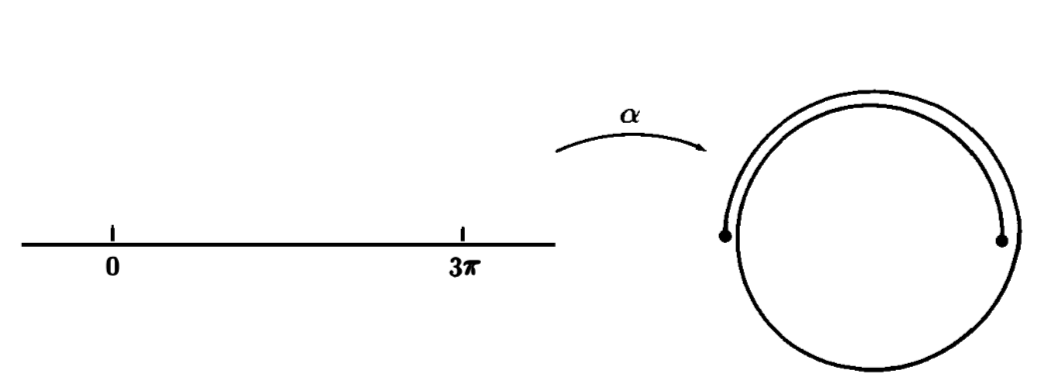
\includegraphics[scale=0.5]{images/Screenshot 2023-01-18 at 16.23.16.png}
        \caption{$\alpha(t)=(a\sin(t),a\cos(t))$ for $0<t<3\pi$}
    \end{figure}
    Although it is useful in physics, we will restrict $\alpha$ to be one-to-one to avoid problems.
\end{itemize}

\begin{definition}
    Let $A$ be open in $\R^2$. Let $\alpha:A\longrightarrow \R^n$ be of class $C^r$. Let $Y=\alpha(A)$.
    Then $Y$ is called a \underline{parametrized-surface} in $\R^n$, and it's 2-dimensional volume is called the \underline{area}
\end{definition}

\begin{theorem}[Area of surface in $\R^3$]
    Let $\alpha:A\subset\R^2\longrightarrow\R^3$ defined as $\alpha(x,y)=(x,y,f(x,y))$, 
    The area of a parametrized-curve in $\R^3$ is given by the formula
    $$v(Y_{\alpha})=\int_A\norm{\frac{\partial \alpha}{\partial x}\times\frac{\partial \alpha}{\partial y}}=\int_A[1+(\frac{\partial f}{\partial x})^2+(\frac{\partial f}{\partial y})^2]^{\frac{1}{2}}$$
    where the symble $\times$ is the cross product.
\end{theorem}
\noindent\textbf{Example}:
\begin{itemize}
    \item Compute the area of a hemisphere in $\R^3$.\\
    Let $\alpha(x,y)=(x,y,f(x,y))$ where $f(x,y)=\sqrt{a^2-x^2-y^2}$ note that $a$ is the radius of the hemisphere. 
    \begin{figure}[ht]
        \centering
        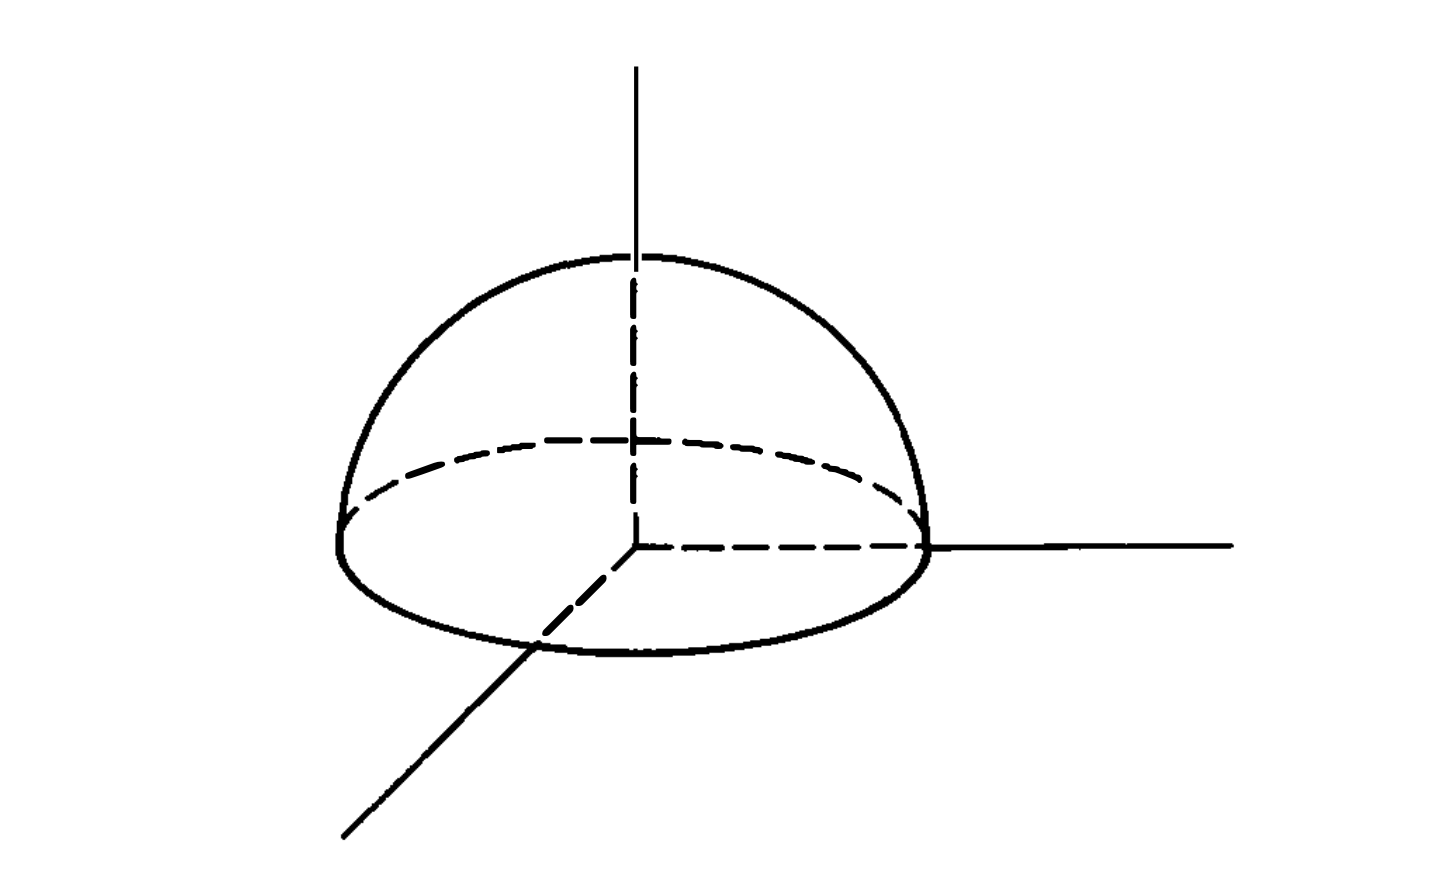
\includegraphics[scale=0.3]{images/Screenshot 2023-01-18 at 20.28.41.png}
        \caption{Picture of a hemisphere}
    \end{figure}
    First, we compute the partial derivatives $$D_1f(x,y)=\frac{-x}{\sqrt{a^2-x^2-y^2}}$$ $$D_2f(x,y)=\frac{-y}{\sqrt{a^2-x^2-y^2}}$$
    By the theorem above $$V(D\alpha(x,y))=[1+(D_1f)^2+(D_2f)^2]^{\frac{1}{2}}=\frac{a}{\sqrt{a^2-x^2-y^2}}$$
    By the definition of integral over $Y_{\alpha}$ with respect to volume, we have 
    $$v(Y_{\alpha})=\int_{Y_{\alpha}}1\di V=\int_{(x,y)\in A}V(D\alpha(x,y))$$
    Let $g:B=(0,a)\times(0,2\pi)\longrightarrow A$ be the polar coordinate transformation. so
    \begin{equation*}
        \begin{split}
            v(Y_{\alpha}) &= \int_{(x,y)\in A}V(D\alpha(x,y))\\
            &= \int_B(V(D\alpha) \circ g)\cdot|\det(Dg)|\\
            &= \int_B\frac{ar}{\sqrt{a^2-(r\cos\theta)^2-(r\sin\theta)^2}}\\
            &= \int_B\frac{ar}{\sqrt{a^2-r^2}}
        \end{split}
    \end{equation*}
    Let $h(r,\theta)=\frac{ar}{\sqrt{a^2-r^2}}$, $h$ is unbouded on $B$, so we must use improper integral. 
    \begin{figure}[ht]
        \centering
        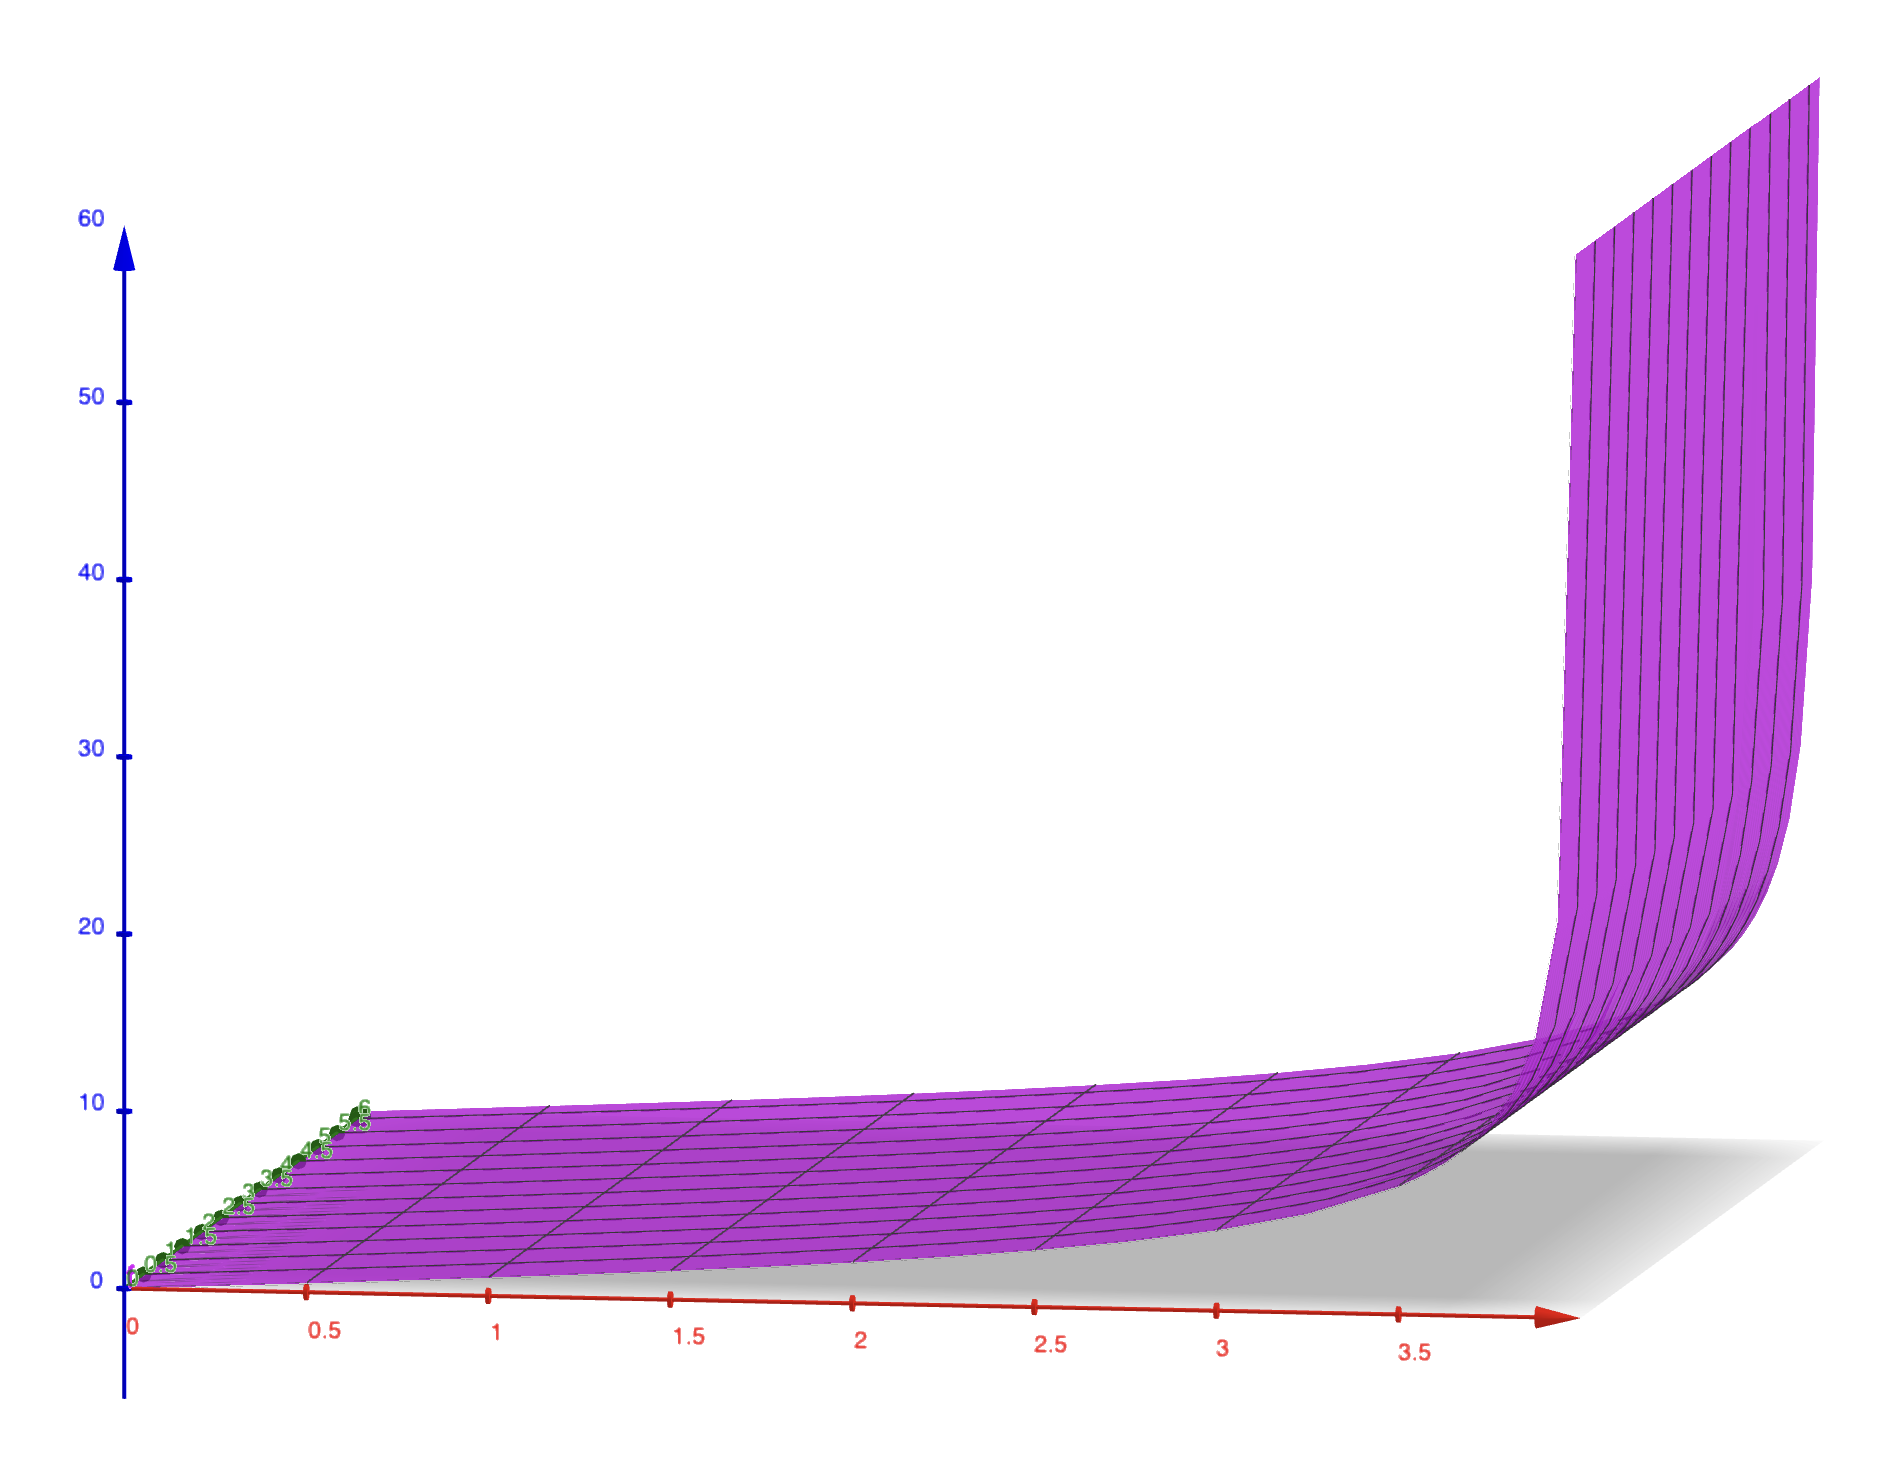
\includegraphics[scale=0.3]{images/Screenshot 2023-01-18 at 19.52.34.png}
        \caption{Picture of $h(r,\theta)$ on the set $B$}
    \end{figure}
    Define 
    $$U_N=(0,a_N)\times(0,2\pi)$$ with $0<a_1<a_2<\cdots<a$ and $\lim_{N\to\infty}a_N=a$.
    Now we can use Fubini theorem on $U_N$.
    \begin{equation*}
        \begin{split}
            \int_{U_N}\frac{ar}{\sqrt{a^2-r^2}} &= \int_{r=0}^{r=a_N}\int_{\theta=0}^{\theta=2\pi}\frac{ar}{\sqrt{a^2-r^2}}\di\theta \di r\\
            &= 2\pi \int_{r=0}^{r=a_N}\frac{ar}{\sqrt{a^2-r^2}}\di r\\
            &= 2\pi(-a\sqrt{a^2-a_N^2}+a\sqrt{a^2})\\
            &= 2\pi(-a\sqrt{a^2-a_N^2}+a^2)
        \end{split}
    \end{equation*}
    Therefore 
    \begin{equation*}
        \begin{split}
            v(Y_{\alpha})&= \lim_{N\to\infty}\int_{U_N}\frac{ar}{\sqrt{a^2-r^2}}\\
            &= \lim_{N\to\infty}2\pi(-a\sqrt{a^2-a_N^2}+a^2)\\
            &= 2\pi a^2
        \end{split}
    \end{equation*}
\end{itemize}

\section{General Manifolds in $\R^n$}

\begin{definition}
    Let $k > 0$. A \underline{k-manifold without boundary} in $\R^n$ of class $C^r$ is a subspace $M\subset \R^n$ having the following property:
    For each $p \in M$, there is an open set $V \subset M$ containing $p$, an open set $U\subset \R^k$ and a continuous bijective map $\alpha: U \longrightarrow V$ such that:
    \begin{itemize}
        \item $\alpha$ is of class $C^r$.
        \item $\alpha^{-1}:V \longrightarrow U$ is continuous.
        \item $D\alpha(x)$ has rank $k$ for each $x \in U$.
    \end{itemize}
    The map $\alpha$ is called a \underline{coordinate patch} on $M$ about $p$.
\end{definition}
\noindent\textbf{Remark}:
\begin{itemize}
    \item In mathematics, a manifold is a topological space that locally resembles Euclidean space near each point.
    \item $rank(D\alpha(x))=k$ means that vectors $D_1\alpha(x),\cdots,D_k\alpha(x)$ are independent at $x$. Geometrically, those vectors span a k-dimensional tangent plane to $M$.
    \begin{figure}[H]
        \centering
        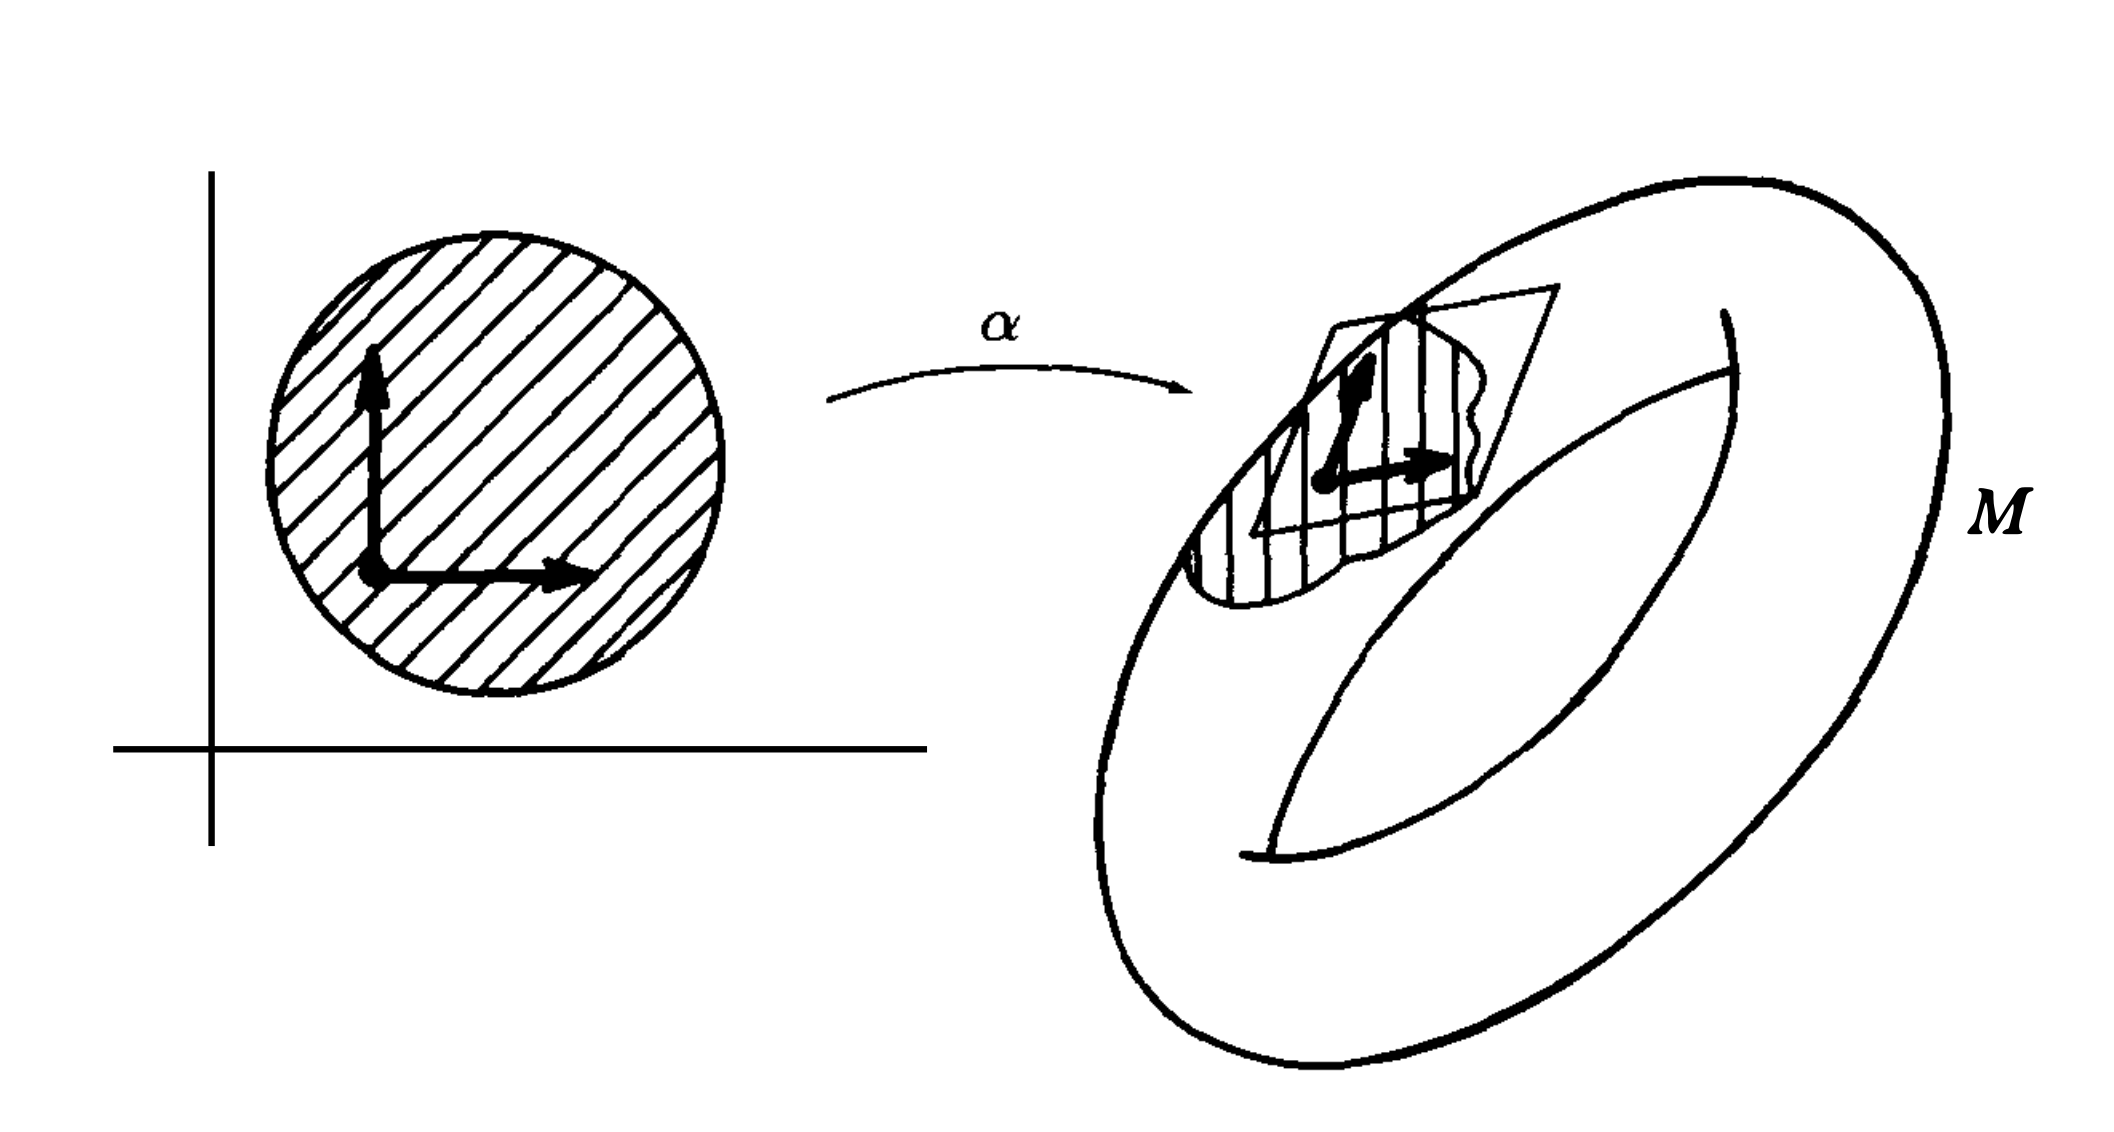
\includegraphics[scale=0.3]{images/Screenshot 2023-01-21 at 19.38.35.png}
        \caption{Meaning of $rank(D\alpha(x))=k$}
    \end{figure}
    Also, this condition means that $M$ does not have cusps or corners. This is a condition that parametrized
    -manifold does not have. 
    \item $\alpha^{-1}$ is continuous means that $\alpha:U\longrightarrow V$ should be a diffeomorphism.
    $M$ has the property that each point has a neighborhood that is homeomorphic(diffeomorphic) to an open subset of n-dimensional Euclidean space.
    While the parametrized-manifold only requirs parametrize the object with a continuous function.
\end{itemize}
\noindent \textbf{Examples}:(Non-examples for manifold without boundary)\\
\begin{itemize}
    \item Let $\alpha:\R\longrightarrow\R^2$ be given by the equation $$\alpha(t)=(t^3,t^2)$$
    Let $M$ be the image of $\R$. We can check that $M$ is a parametrized-manifold of dimension 1.
    \begin{figure}[H]
        \centering
        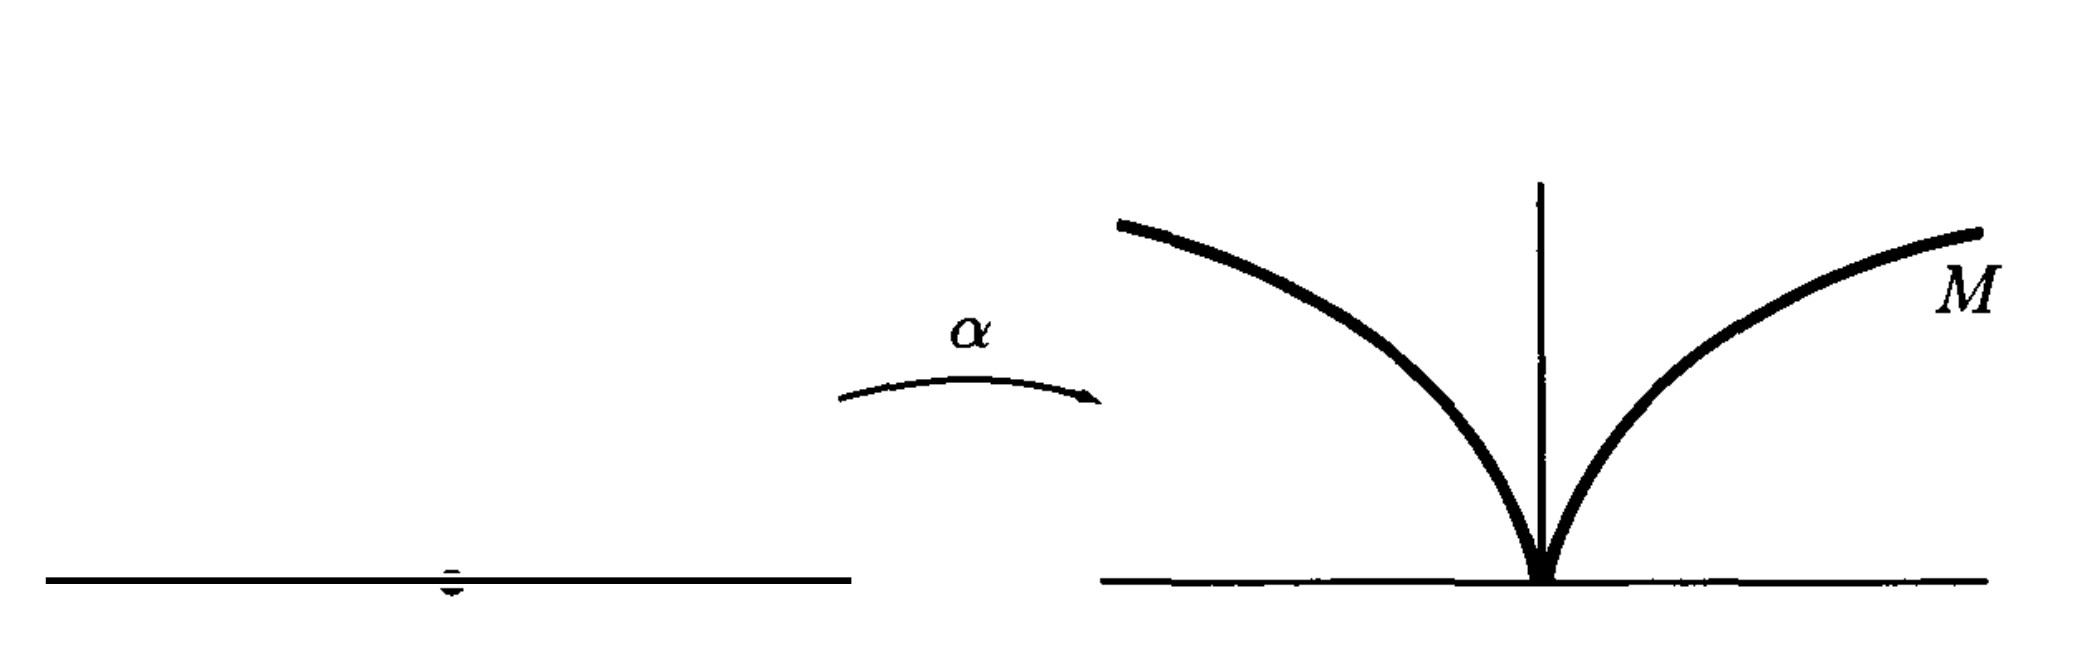
\includegraphics[scale=0.3]{images/Screenshot 2023-01-21 at 19.50.40.png}
        \caption{$\alpha(t)=(t^3,t^2)$}
    \end{figure}
    Also, $\alpha,\alpha^{-1}$ are continuous, $\alpha$ is of class $C^{\infty}$. But $rank(D\alpha(0))=0$, the picture shows that $M$ has a cusp at $0$. $M$ is not a manifold wihout boundary.
    
    \item Let $\alpha:\R^2\longrightarrow\R^3$ be given by the equation $$\alpha(x,y)=(x(x^2+y^2),y(x^2+y^2),x^2+y^2)$$
    Let $M$ be the image of $\R^2$. We can check that $M$ is a parametrized-manifold of dimension 2.
    \begin{figure}[H]
        \centering
        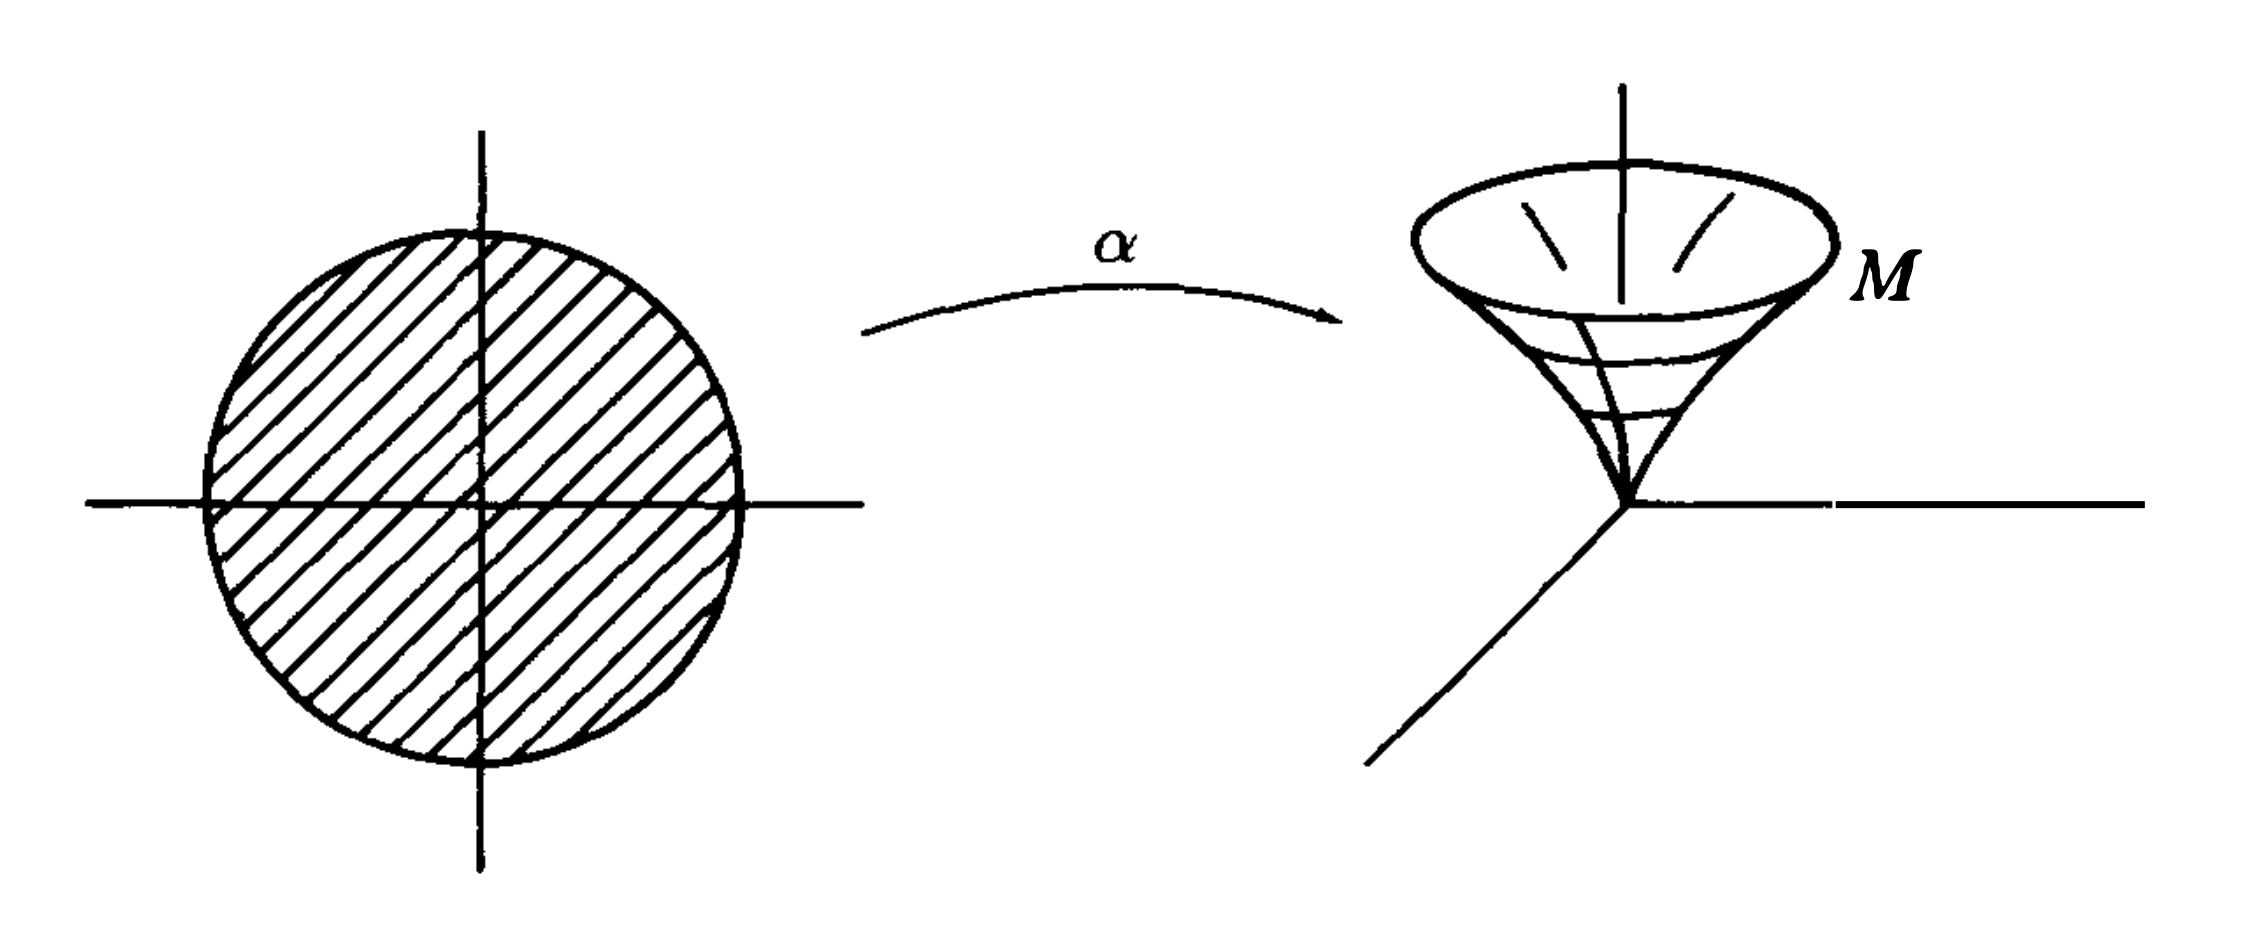
\includegraphics[scale=0.3]{images/Screenshot 2023-01-21 at 20.14.15.png}
        \caption{$\alpha(x,y)=(x(x^2+y^2),y(x^2+y^2),x^2+y^2)$}
    \end{figure}
    Also, $\alpha,\alpha^{-1}$ are continuous, $\alpha$ is of class $C^{\infty}$. But $rank(D\alpha(0))=0$, the picture shows that $M$ has a cusp at $0$. 
    In other words, $M$ fails to have a tangent plane at the origin. 
    $M$ is not a manifold wihout boundary.

    \item Let $\alpha:(0,\pi)\longrightarrow\R^2$ be given by the equation $$\alpha(t)=(\sin(2t)|\cos(t)|,\sin(2t)\sin(t))$$
    Let $M$ be the image of $(0,\pi)$. We can check that $M$ is a parametrized-manifold of dimension 1.
    \begin{figure}[H]
        \centering
        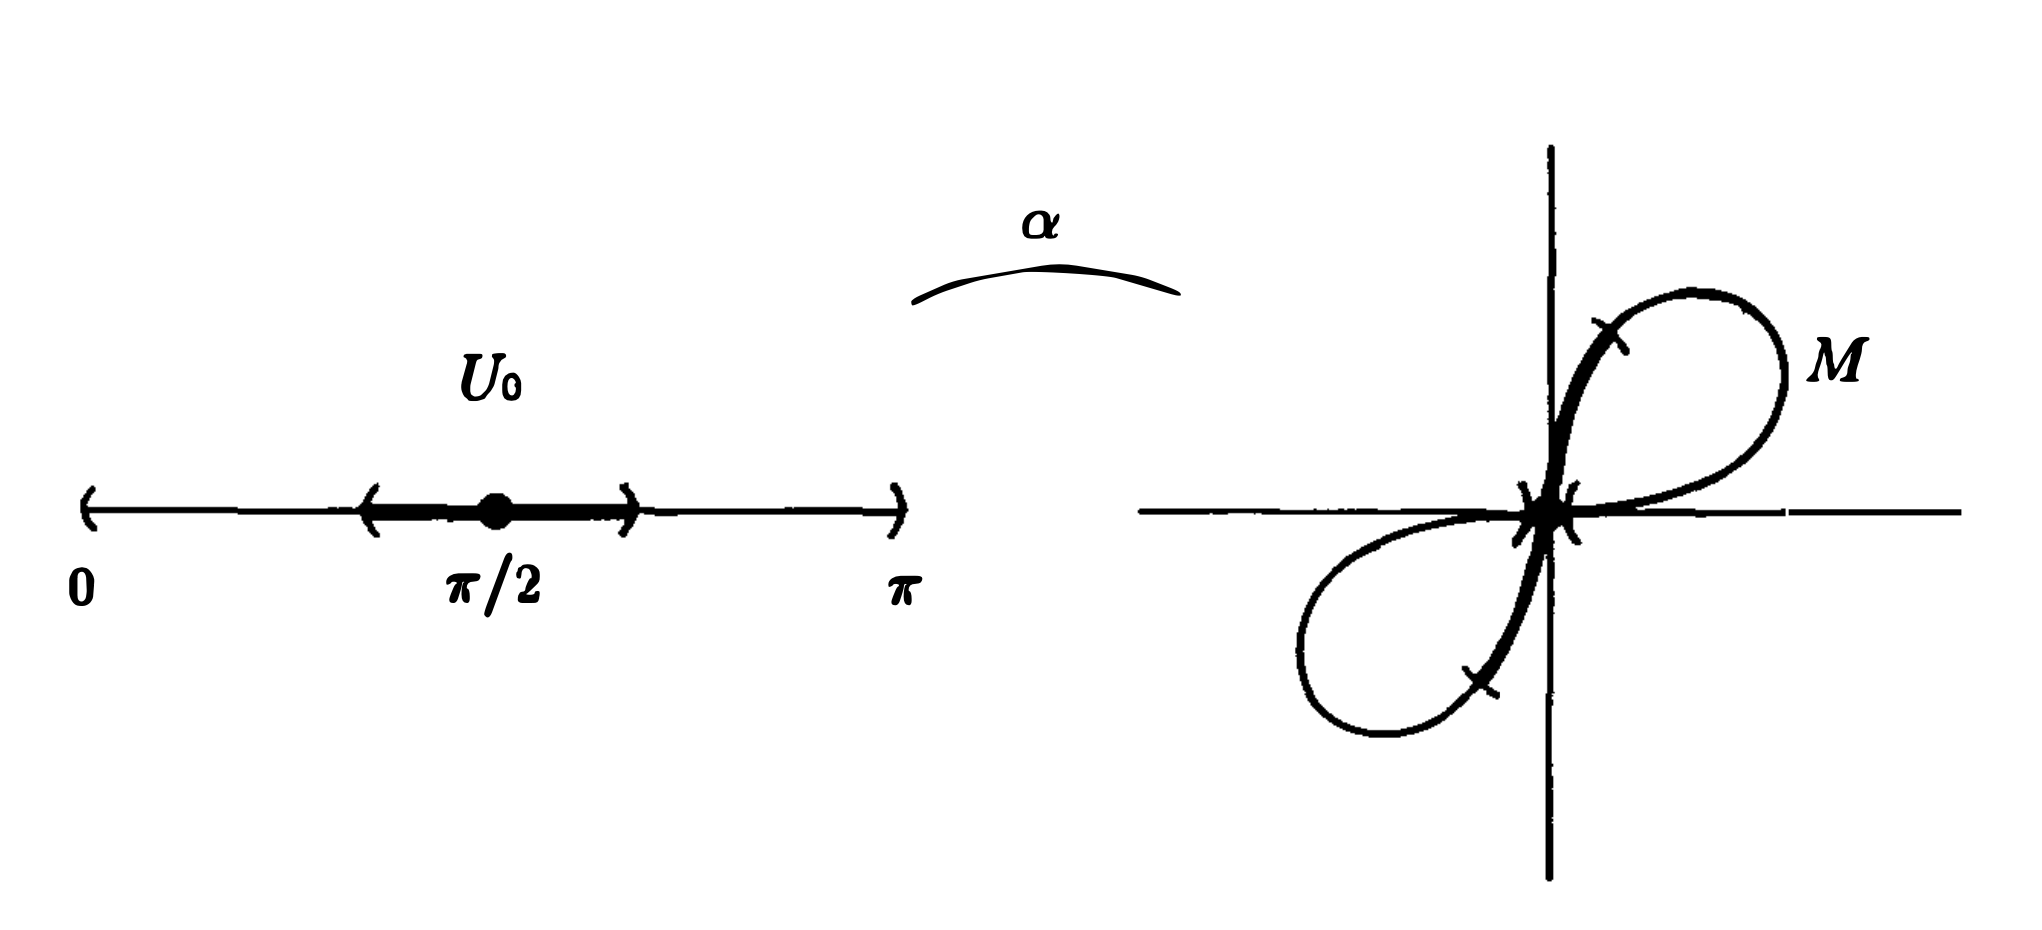
\includegraphics[scale=0.3]{images/Screenshot 2023-01-21 at 20.22.38.png}
        \caption{$\alpha(t)=(\sin(2t)|\cos(t)|,\sin(2t)\sin(t))$}
    \end{figure}
    This time, $\alpha$ is continuous and $rank(D\alpha)=1$ for all $x\in(0,\pi)$. But $\alpha^{-1}:M \longrightarrow(0,\pi)$ is not continuous.
    Let $U_0$ be an open set around $\frac{\pi}{2}$ in $(0,\pi)$ the preimage of $U_0$ under $\alpha^{-1}$ is not open in $M$.
\end{itemize}

\begin{theorem}
    Let $Y_{\alpha}$ be a parametrized-manifold with $\alpha:A\longrightarrow \R^n$. 
    If $\alpha^{-1}$ is continuous and $D\alpha$ has rank $k$, then $Y$ is a manifold without boundary. 
    In this case, $Y$ is covered by a single coordinate patch $\alpha$.
\end{theorem}

\begin{definition}
    Let $S$ be a subset of $\R^k$. Let $f:S\longrightarrow\R^n$. We say $f$ is \underline{of class $C^r$ on $S$} if $f$ may be extended to a function $g:U\longrightarrow\R^n$ that is of class $C^r$ on an open set $U$ of $\R^k$ containing $S$.
\end{definition}

\begin{theorem}
    By adopting the definition above, the composition of functions of class $C^r$ is of class $C^r$.
\end{theorem}

\begin{lemma}
    Let $f:S\subset\R^k\longrightarrow\R^n$. If for each $x\in S$, there is a neighborhood $U_x$ of $x$ such that $f|_{U_x\cap S}$ is of class $C^r$ on $U_x\cap S$, then $f$ is of class $C^r$ on $S$.
\end{lemma}

\begin{definition}\
    \begin{itemize}
        \item Let $\HH^k$ denote the \underline{upper half-space} in $\R^k$, consisting of those $x\in \R^k$ with $x_k\geq 0$.
        \item Let $\HH^k_+$ denote the \underline{open upper half-space} in $\R^k$, consisting of those $x\in \R^k$ with $x_k> 0$.
    \end{itemize}
\end{definition}
\noindent\textbf{Remark}:
\begin{itemize}
    \item We shall be particularly interested in functions defined on sets that are open in $\HH^k$ but not in $\R^k$.
\end{itemize}

\begin{lemma}
    Let $U$ be open in $\HH^k$. Let $\alpha:U\longrightarrow\R^n$ be of class $C^r$. Let $\beta:U'\longrightarrow\R^n$ be of class $C^r$ be an extension of $\alpha$ defined on an open set $U'\subset \R^k$. 
    Then $$\forall x\in U.D\beta(x)=D\alpha(x)$$
\end{lemma}

\begin{definition}
    Let $k > 0$. A \underline{k-manifold} in $\R^n$ of class $C^r$ is a subspace $M\subset \R^n$ having the following property:
    For each $p \in M$, there is an open set $V \subset M$ containing $p$, a set $U\subset \R^k$ that is either open in $\R^k$ or $\HH^k$, and a continuous bijective map $\alpha: U \longrightarrow V$ such that:
    \begin{itemize}
        \item $\alpha$ is of class $C^r$.
        \item $\alpha^{-1}:V \longrightarrow U$ is continuous.
        \item $D\alpha(x)$ has rank $k$ for each $x \in U$.
    \end{itemize}
    The map $\alpha$ is called a \underline{coordinate patch} on $M$ about $p$.
\end{definition}
\noindent\textbf{Remark}:
\begin{itemize}
    \item We extend the definition to the case $k=0$ by declaring a discrete collection of points in $\R^n$ to be a \underline{0-manifold} in $\R^n$.
    \item The difference of this definition and the definition of manifold without boundary is the set $U$ can be open in $\HH^k$. So the points which have neighborhoods that look like open half-balls in $\HH^k$ instead of open balls in $\R^k$ shall called the boundary of $M$. Consider the following picture.
    \begin{figure}[H]
        \centering
        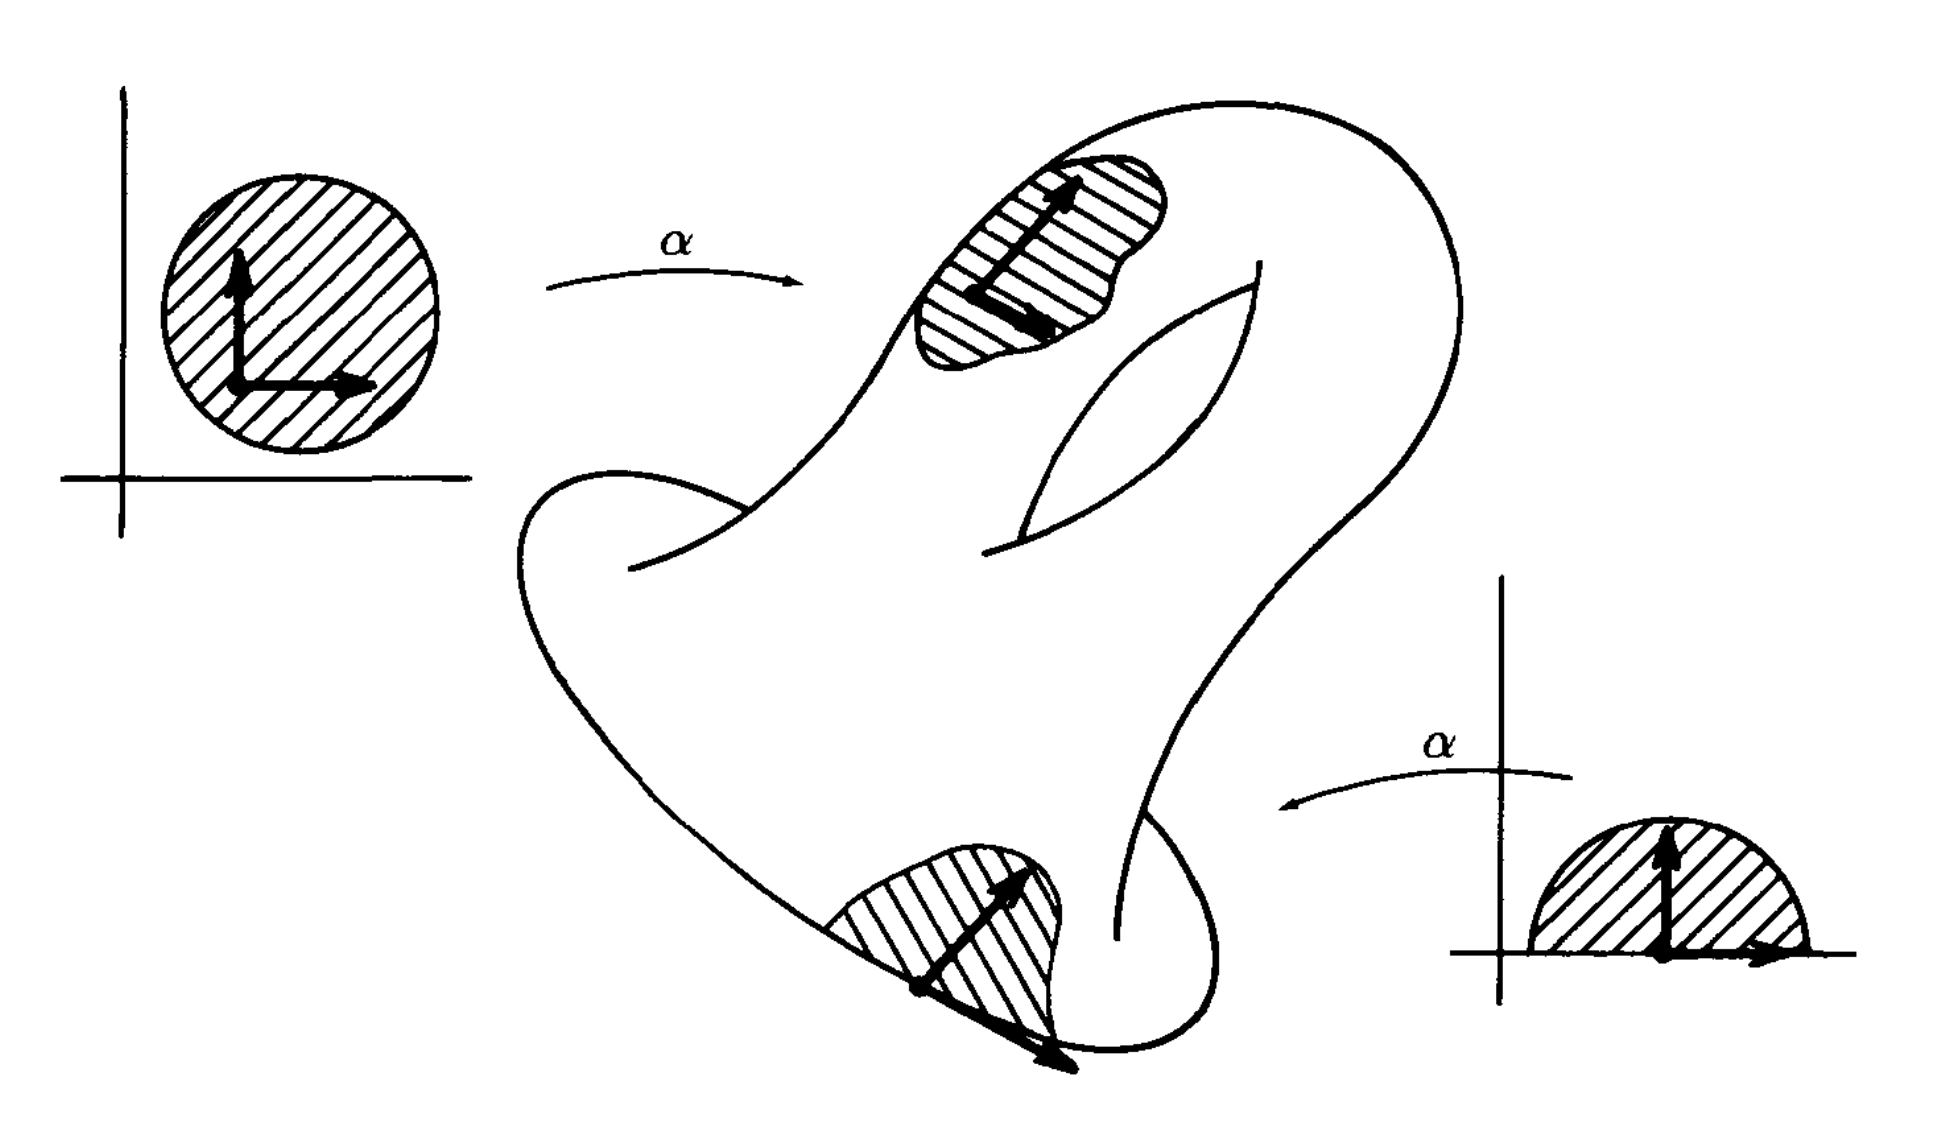
\includegraphics[scale=0.3]{images/Screenshot 2023-01-21 at 21.38.04.png}
        \caption{A picture of 2-manifold in $\R^3$}
    \end{figure}
    We will make this definition rigorous in the next section.
\end{itemize}

\begin{lemma}
    Let $M$ be a manifold in $\R^n$. Let $\alpha:U\longrightarrow V$ be a coordinate patch on $M$. If $U_0$ is a subset of $U$ that is open in $U$, then the restriction of $\alpha$ to $U_0$ is also a coordinate patch on $M$.
\end{lemma}

\section{The Boundary of a Manifold}

\begin{theorem}\label{transition function thm}
    Let $M$ be a k-manifold in $\R^n$ of class $C^r$. Given two coordinate patches $$\alpha_0:U_o\longrightarrow V_0$$ $$\alpha_1:U_1\longrightarrow V_1$$
    with the intersection $W=V_0\cap V_1\neq \emptyset$. Let $W_i=\alpha_i^{-1}(W)$. Then the map $$\alpha_1^{-1}\circ \alpha_0:W_0\longrightarrow W_1$$
    is of class $C^r$, and its derivative is non-singular. We call the function $\alpha_1^{-1}\circ \alpha_0$ \underline{transition function}.
\end{theorem}

\noindent\textbf{Remark}:
\begin{itemize}
    \item Since the sets $U_i$ are open in $\R^k$ or $\HH^k$. So we have three types of transitions as shown in the graph.
    \begin{figure}[H]
        \centering
        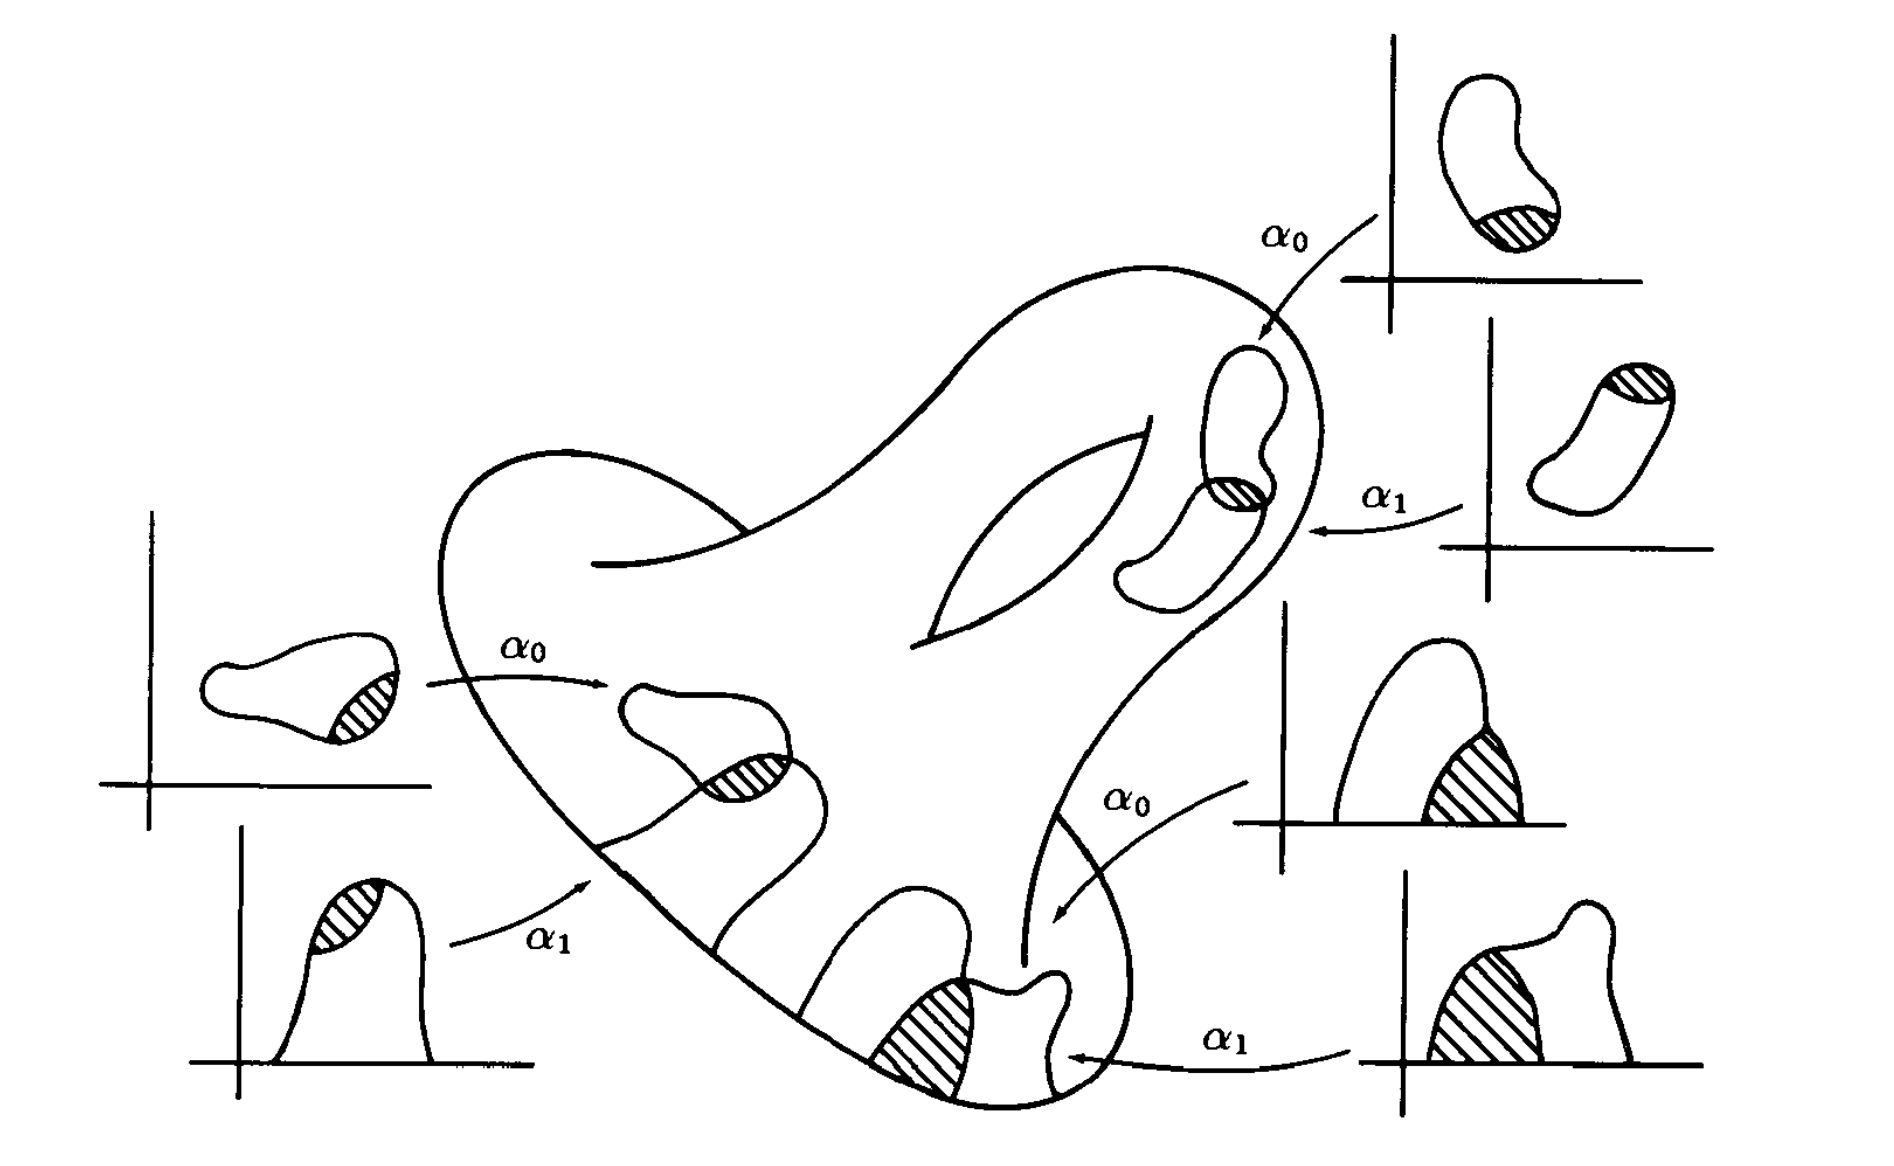
\includegraphics[scale=0.35]{images/Screenshot 2023-01-30 at 15.07.28.png}
        \caption{Three types of transition functions}
    \end{figure}
    \item In the future, we will study the manifold that does not live in $\R^n$, and this theorem will be very important to define such manifold.
\end{itemize}

\begin{definition}
    Let $M$ be a k-manifold in $\R^n$. Let $p\in M$.
    \begin{itemize}
        \item If there exists a coordinate patch $\alpha:U\longrightarrow V$ on $M$ about $p$ such that $U$ is open in $\R^k$, we say $p$ is an \underline{interior point} of $M$.
        \item If not, we say $p$ is a \underline{boundary point} of $M$. 
    \end{itemize}
    We denote the set of boundary points of $M$ by $\partial M$, and call this set the \underline{boundary} of $M$. 
\end{definition}
\noindent\textbf{Remark}:
\begin{itemize}
    \item The interior points and boundary points of the manifold $M$ has nothing to do with the term interior and boundary in general topology.
    \item Consider the $S^2$ in $\R^3$, all points in $S^2$ are interior points of the manifold $S^2$. But it is clear that $Int(S^2)=\emptyset$ because for any $p\in S^2.$ we cannot find any open ball of $x$ contained in $S^2$, hence all points in $S^2$ are in the boundary of $S^2$.
\end{itemize}

\begin{lemma}[Identify boundary points]
    Let $M$ be a k-manifold. Let $\alpha:U\longrightarrow V$ be a coordinate patch about the point $p\in M$.
    \begin{itemize}
        \item If $U$ is open in $\R^k$, then $p$ is an interior point.
        \item If $U$ is open in $\HH^k$ and $p=\alpha(x_0)$ for $x_0\in \HH^k_+$, then $p$ is an interior of $M$.
        \item If $U$ is open in $\HH^k$ and $p=\alpha(x_0)$ for $x_0\in \R^{k-1}\times 0$, then $p$ is a boundary point of $M$.
    \end{itemize}
\end{lemma}

\begin{theorem}
    Let $M$ be a k-manifold in $\R^n$ of class $C^r$. If $\partial M$ is non-empty, then $\partial M$ is a k-1 manifold without boundary in $\R^n$ of class $C^r$.
\end{theorem}

\begin{theorem}
    Let $\mathcal{O}$ be open in $\R^n$. Let $f:\mathcal{O}\longrightarrow \R$ be of class $C^r$. 
    Let $M$ be the set of points $x$ for which $f(x)=0$. Let $N$ be the set of points for which $f(x)\geq0$. 
    Suppose $M$ is non-empty and $\forall x \in M.rank(Df(x))=1$. Then $N$ is an n-manifold in $\R^n$ and $\partial N=M$.
\end{theorem}
\noindent\textbf{Example}:
\begin{itemize}
    \item The n-ball $B^n(a)$ is an n-manifold in $\R^n$ of class $C^{\infty}$ and $\partial B^n(a)=S^{n-1}(a)$ which is the (n-1)-sphere.\\ 
    We apply the preceding theorem to the function $$f(x)=a^2-\norm{x}^2=a^2-(x_1)^2-\cdots-(x_n)^2$$
    Hence we can compute the derivative of $f$ $$Df(x)=\begin{bmatrix}
        (-2x_1) & \cdots & (-2x_n)
    \end{bmatrix}$$
    This matrix has rank 1 at each points of $S^{n-1}(a)$.
    \item The  solid torus $T$ is a 3-manifold, and its boundary is the torus.\\
    Let $g$ be the cylindrical coordinate transformation. Let $$A=\{(r,\theta,z):(r-b)^2+z^2\leq a^2\text{ and }0\leq \theta\leq 2\pi\}$$
    Recall the previous example, the \underline{Solid Torus} $T$ is the image of $A$ under $g$. We define $f:\R^3\longrightarrow\R$ as $$f(x,y,x)=a^2-(\sqrt{x^2+y^2}-b)^2-z^2$$
    Intuitively, $f$ is the square of the distance of point $(x,y,z)$ to the torus $\partial T$. By computation, 
    $$Df(x,y,z)=\begin{bmatrix}
        -2x+\frac{2xb}{\sqrt{x^2+y^2}}& -2y+\frac{2yb}{\sqrt{x^2+y^2}}&-2z
    \end{bmatrix}$$
    We need to show that $rank(Df(x,y,z))=1$ whenever $f(x,y,z)=0$. This is equivalent to proving the contrapositive statement: 
    $$rank(Df(x,y,z))\neq1\implies f(x,y,z)\neq0$$
    Suppose $rank(Df(x,y,z))\neq1$, then it must be 0. Hence $x^2+y^2=b^2$ and $z=0$. Therefore $f(x,y,z)=a^2>0$.
\end{itemize}

\begin{theorem}
    Let $f:\R^{n+k}\longrightarrow\R^n$ be of class $C^r$. Let $M=\{x\in \R^{n+k}:f(x)=0\}$. Suppose $M$ is non-empty and $\forall x\in M.rank(Df(x))=n$, then we have
    \begin{enumerate}
        \item $M$ is a k-manifold without boundart in $\R^{n+k}$.
        \item If $N=\{x\in\R^{n+k}:f_1(x)=\cdots=f_{n-1}(x)\text{ and }f_n(x)\geq 0\}$ and $$\forall x \in N.rank(D(f_1,\cdots,f_{n-1})(x))=n-1$$
        Then $N$ is a (k+1)-manifold and $\partial N=M$.
    \end{enumerate}
\end{theorem}
\noindent\textbf{Remark}:
\begin{itemize}
    \item The solution of the equation $f(x)=(f_1(x),\cdots,f_n(x))=\vec{0}$ can be thought as the intersection of hyper-surfaces $f_i(x)=0$. If the condition of the theorem above is satisfied, then $f_1(x)=0$ is a (n+k-1)-manifold, when it intersects $f_2(x)=0$, the dimension will minuse 1. After intersects $f_n(x)=0$, we intersects $n-1$ times, Hence $M$ has dimension $n+k-1-(n-1)=k$.
    \item for example, let $f,g:\R^3\longrightarrow\R$ be of class $C^r$. Let $M\neq \emptyset$ be the solution set of the system of equations \begin{equation*}
        \begin{cases}
            f(x,y,z)=0\\
            g(x,y,z)=0
        \end{cases}
    \end{equation*}
    Define $h=(f,g):\R^3\longrightarrow\R^2$. If we have the condition that $$\forall x\in M.rank(Dh(x))=2$$
    Then $M$ is a 1-manifold without boundary in $\R^3$. In other words, the solution set is a smooth curve without singularities.
\end{itemize}

\section{Integral of Scalar Functions over Manifold}

\begin{definition}
    Let $M$ be a compact k-manifold in $\R^n$ of class $C^r$. Let $f:M\longrightarrow\R^n$ be a continuous function. Let $C=supp(f)$. $C$ is compact beacause $C$ is closed in compact space $M$. Suppose $C$ can be covered by a single coordinate patch. i.e. $$\exists \text{ coordinate patch }\alpha:U\longrightarrow V.\text{such that }C\subset V$$
    Now $\alpha^{-1}(C)$ is compact in $\R^k$. Therefore, by replacing $U$ by a smaller open set if necessary, we can assume that $U$ is bounded. we define the \underline{integral of $f$ over $M$} by 
    $$\int_Mf\di V=\int_{Int(U)}(f\circ \alpha)V(D\alpha)$$
    \begin{itemize}
        \item If $U$ is open in $\R^k$, then $Int(U)=U$.
        \item If $U$ is open in $\HH^k$ but not open in $\R^k$, then $Int(U)=U\cap\HH^k_+$.
    \end{itemize}
\end{definition}
\noindent\textbf{Remark}:
\begin{itemize}
    \item The function $F=(f\circ\alpha)V(D\alpha)$ is continuous on bounded $U$ and vanish outside the compact set $\alpha^{-1}(C)$, hence $F$ is bounded.
    If $U$ is open in $\R^k$ , then $F$ vanishes near each point of $Bd(U)$. If $U$ is not open in $\R^k$, then $F$ vanishes near near each point of $Bd(U)$ not in $\partial \HH^k$. In either case, 
    $F$ is integrable over $U$ and hence over $Int(U)$.
    \begin{figure}[H]
        \centering
        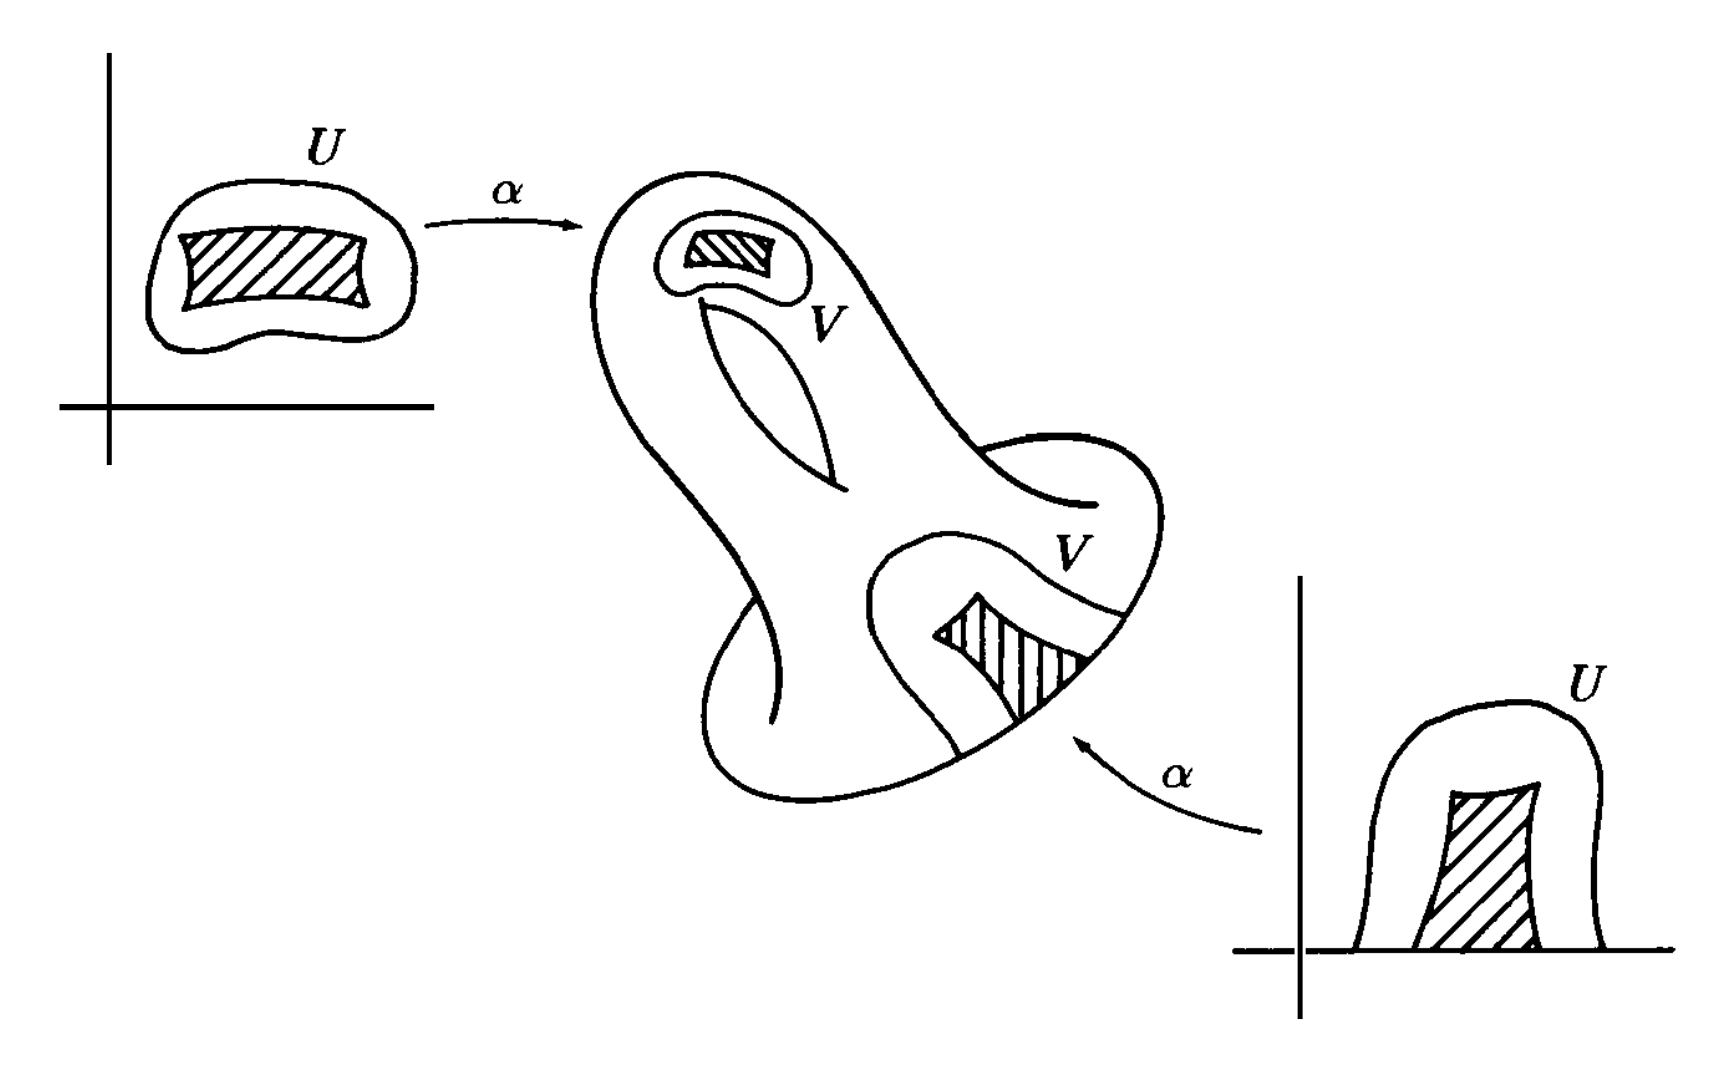
\includegraphics[scale=0.3]{images/Screenshot 2023-02-07 at 22.27.15.png}
    \end{figure}
    \item This integral exists as an ordinary integral, and hence as an extended integral.
\end{itemize}

\begin{lemma}
    If the support of $f$ can be covered by a single coordinate patch, the integral $\int_Mf\di V$ is well-defined, independent of the choice of coordinate patch.
\end{lemma}

\begin{theorem}[existence of finite partition of unity on $M$]
    Let $M$ be a compact k-manifold in $\R^n$ of class $C^r$. Given a covering of $M$ by coordinate patches, there exists a finite collection of $C^{\infty}$ functions $\phi_1,\cdots,\phi_l:\R^n\longrightarrow[0,1]$ such that
    \begin{enumerate}
        \item Given $i$, the support of $\phi_i$ is compact and there is a coordinate patch $\alpha_i:U_i\longrightarrow V_i$ belonging to the given covering such that $$(supp(\phi_i)\cap M)\subset V_i$$
        \item $\sum\phi_i(x)=1$ for $x\in M$.
    \end{enumerate}
    We call $\{\phi_1,\cdots,\phi_l\}$ a \underline{partition of unity on $M$} dominated by the given collecction of coordinate patches. 
\end{theorem}

\begin{definition}
    Let $M$ be a compact k-manifold in $\R^n$ of class $C^r$. Let $f:M\longrightarrow \R$ be continuous. 
    Choose a partition of unity $\{\phi_1,\cdots,\phi_l\}$ on $M$ that is dominated by the collection of all coordinate patches on $M$. 
    We define the \underline{inegral of $f$ over $M$} by the equation 
    $$\int_Mf\di V=\sum_{i=1}^l[\int_M(\phi_if)\di V]$$
    Then we define the \underline{k-dimensional volume of $M$} by the equation 
    $$v(M)=\int_M1\di V$$
\end{definition}
\noindent\textbf{Remark}:
\begin{itemize}
    \item Clearly, this is a more general definition. If the support of $f$ happens to lie in a single coordinate patch $\alpha:U\longrightarrow supp(f)\subset V$, this definition agrees with the preceding definition.
    \begin{equation*}
        \begin{split}
            \sum_{i=1}^l[\int_M(\phi_if)\di V] &= \sum_{i=1}^l[\int_{Int(U)}(\phi_if\circ \alpha)V(D\alpha)] \text{\quad by definition}\\
            &= \int_{Int(U)}[\sum_{i=1}^l(\phi_if\circ \alpha)V(D\alpha)] \text{\quad by linearity}\\
            &= \int_{Int(U)}[\sum_{i=1}^l(\phi_i\circ \alpha)(f\circ \alpha)V(D\alpha)]\\
            &= \int_{Int(U)}(f\circ\alpha)V(D\alpha)\text{\quad because\quad} \sum_{i=1}^l(\phi_i\circ\alpha)=1 \text{ on $A$}\\
            &= \int_Mf\di V \text{\quad by definition}
        \end{split}
    \end{equation*}
    \item What if $supp(f)$ is not contained in a single coordinate patch? Suppose $supp(f)$ is contained in $\{\alpha_1,\cdots,\alpha_t\}$ where $\alpha_i:U_i\longrightarrow V_i$.
    \begin{itemize}
        \item For $\alpha_1:U_1\longrightarrow V_1$, we keep it unchanged. Set $U_1'=U_1,V_1'=V_1$.
        \item For $\alpha_2$, we restrict it as $\alpha_2\big|^{V_2\setminus V_1}$, say $\alpha_2:U_2'\longrightarrow V_2'$.
        \item For $\alpha_k$, we restrict it as $\alpha_k\big|^{V_k\setminus V_{k-1}'}$, say $\alpha_2:U_k'\longrightarrow V_k'$.
    \end{itemize}
    After this process, we get $\{V_1'\cdots,V_t'\}$, which is a partition of $supp(f)$.For each part $V_k'$ of the manifold $M$, with similar argument we get
    $$\sum_{i=1}^l[\int_{V_k'}(\phi_if)\di V]=\int_{V_k'}f\di V$$
    Therefore we have 
    \begin{equation*}
        \begin{split}
            \sum_{i=1}^l[\int_M(\phi_if)\di V] &= \sum_{i=1}^l\sum_{k=1}^t[\int_{V_k'}(\phi_if)\di V]\\
            &= \sum_{k=1}^t\sum_{i=1}^l[\int_{V_k'}(\phi_if)\di V]\\
            &= \sum_{k=1}^t\int_{V_k'}f\di V\\
            &= \int_Mf\di V
        \end{split}
    \end{equation*}
    \item Also notice that this definition is independent of the choice of the partition of unity. Let $\{\psi_1,\cdots,\psi_m\}$ be another choice for the partition of unity. 
    Since $$supp(\psi_jf)\subset supp(\psi_j)\cap supp(f)\subset supp(\psi_j)\cap M\subset V_j$$ where $\psi_j:U_j\longrightarrow V_j$ this means that the support of $\psi_jf$ lies in a single coordinate patch. With similar argument (replacing $f$ by $\psi_jf$) we have 
    $$\sum_{i=1}^l[\int_M(\phi_i\psi_jf)\di V]=\int_M(\psi_jf)\di V$$ 
    Summing over $j$ we get 
    \begin{equation*}
        \begin{split}
            \sum_{j=1}^m\sum_{i=1}^l[\int_M(\phi_i\psi_jf)\di V] &= \sum_{j=1}^m\int_M(\psi_jf)\di V\\
            &= \int_Mf\di V\\
            &= \sum_{i=1}^l[\int_M(\phi_if)\di V]
        \end{split}
    \end{equation*}
\end{itemize}

\begin{theorem}
    Let $M$ be a compact k-manifold in $\R^n$ of class $C^r$. Let $f,g:M\longrightarrow \R$ be continuous. Then 
    $$\int_M(af+bg)\di V =a \int_M f\di V + b\int_M g \di V$$
\end{theorem}
\noindent\textbf{Remark}:
\begin{itemize}
    \item Using partition of unity to define the integral of $f$ over compact manifold $M$ is satisfactory for theoretical purposes, but not for practical purposes. 
    \item For example, if we want to integrate a function over $S^{n-1}$, no one want to actually find a partition of unity on $S^{n-1}$. Instead, we break $S^{n-1}$ into pieces and integrate over each pieces separatelt then add the results together.
\end{itemize}

\begin{definition}
    Let $M$ be a compact k-manifold in $\R^n$ of class $C^r$. A subset $D\subset M$ is said to have \underline{measure zero in $M$} if $D$ can be covered by countably many coordinate patches $\alpha_i:U_i\longrightarrow V_i$ such that the set $$D_i=\alpha_i^{-1}(D\cap V_i)$$ has measure zero in $\R^k$ for each $i$. 
\end{definition}

\begin{theorem}[Equivalent definition of measure zero in $M$]
    $D\subset M$ has measure zero in compact k-manifold $M$ if and only if for any coordinate patch $\alpha:U\longrightarrow V$ on $M$, the set $\alpha^{-1}(D\cap V)$ has measure zero in $\R^k$.
\end{theorem}

\begin{theorem}
    Let $M$ be a compact k-manifold in $\R^n$ of class $C^r$. Let $f:M\longrightarrow \R$ be continuous. Suppose we have coordinate patches $\{\alpha_1,\cdots,\alpha_N\}$ where $\alpha_i:A_i\longrightarrow M_i$ such that $A_i$ is open in $\R^k$. Also, $\{M_1,\cdots,M_N,K\}$ is a partition of $M$ where $K$ has measure zero in $M$. Then
    $$\int_Mf\di V=\sum_{i=1}^N[\int_{A_i}(f\circ\alpha_i)V(D\alpha_i)]$$
\end{theorem}
\noindent\textbf{Remark}:
\begin{itemize}
    \item This theorem is for practical purposes. And it says that $\int_Mf\di V$ can be evaluated by breaking $M$ up into pieces that are parametrized-manifolds and integrating $f$ over each piece separately.
\end{itemize}
\noindent\textbf{Example}:
\begin{itemize}
    \item Alternate method for computing the area of $S^2(a)$.\\
    Recall that we think the upper hemisphere with radius $a$ as a parametrized-manifold and used improper integral to get the area of the upper hemisphere is $2\pi a^2$. Hence the area of $S^2(a)$ is $4\pi a^2$. 
    Given $z_0\in \R$ with $|z_0|<a$, the intersection of $S^2(a)$ with the plane $z=z_0$ is the circle 
    $$\{(x,y,z)\in S^2(a): x^2+y^2=a^2-(z_0)^2\text{ and }z=z_0\}$$
    This fact suggests that we parametrize $S^2(a)$ by the function $\alpha:A\longrightarrow \R^3$
    $$\alpha(t,z)=(\sqrt{a^2-z^2}\cos(t), \sqrt{a^2-z^2}\sin(t), z)$$
    where $A$ is the set 
    $$A=\{(t,z)\in \R^2: 0<t<2\pi \text{ and }|z|<a\}$$
    \begin{figure}[H]
        \centering
        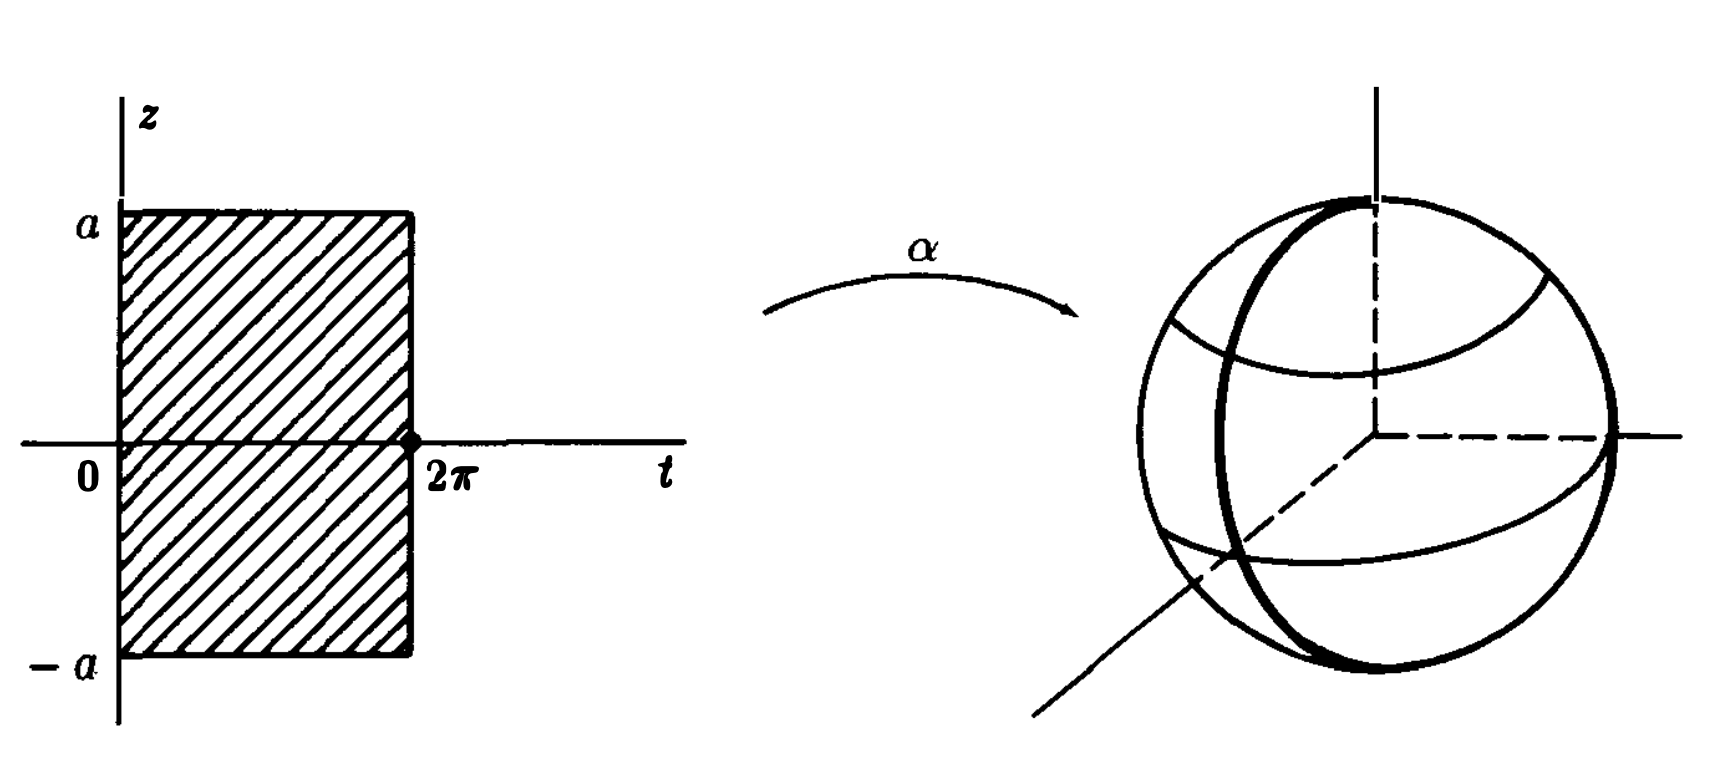
\includegraphics[scale=0.3]{images/Screenshot 2023-02-27 at 22.11.04.png}
    \end{figure}
    As shown in the picture that $\alpha$ is a coordinate patch that covers all of $S^2(a)$ except for a great-circle arc, which has measure zero in $S^2(a)$.
    Sicne \begin{equation*}
        D\alpha=\begin{bmatrix}
            -\sqrt{a^2-z^2}\sin(t) & \frac{-z\cos(t)}{\sqrt{a^2-z^2}}\\
            \sqrt{a^2-z^2}\cos(t) & \frac{-z\sin(t)}{\sqrt{a^2-z^2}}\\
            0 & 1
        \end{bmatrix}
    \end{equation*}
    By brutal computation we have $V(D\alpha)=\sqrt{\det(D^T\alpha\cdot D\alpha)}=a$, Therefore
    \begin{equation*}
        v(S^2(a))= \int_A1V(D\alpha)=\int_Aa=4\pi a^2
    \end{equation*}
\end{itemize}

\begin{theorem*}
    Let $M$ and $N$ be compact manifolds without boundary in $\R^m$ and $\R^n$ respectively. Let $f:M\longrightarrow \R$ and $g:N\longrightarrow \R$ be continuous. Then 
    $$\int_{M\times N}f\cdot g \di V=[\int_Mf\di V][\int_Ng\di V]$$
    It followa that $$v(M\times N)=v(M)\times v(N)$$
\end{theorem*}
\noindent\textbf{Example}:
\begin{itemize}
    \item In topology, we know that the torus is homeomorphic to $S^1\times S^1$. But what is $S^1\times S^1$? It is a 2-manifold in $\R^4$ and we can now compute the area of $S^1\times S^1$
    $$v(S^1\times S^1)=v(S^1)\times v(S^1)=(2\pi)^2$$
\end{itemize}